%% (Master) Thesis template
% Template version used: v1.4
%
% Largely adapted from Adrian Nievergelt's template for the ADPS
% (lecture notes) project.


%% We use the memoir class because it offers a many easy to use features.
\documentclass[11pt,a4paper]{memoir}

%% Packages
%% ========

%% LaTeX Font encoding -- DO NOT CHANGE
\usepackage[OT1]{fontenc}

%% Babel provides support for languages.  'english' uses British
%% English hyphenation and text snippets like "Figure" and
%% "Theorem". Use the option 'ngerman' if your document is in German.
%% Use 'american' for American English.  Note that if you change this,
%% the next LaTeX run may show spurious errors.  Simply run it again.
%% If they persist, remove the .aux file and try again.
\usepackage[english]{babel}

%% Input encoding 'utf8'. In some cases you might need 'utf8x' for
%% extra symbols. Not all editors, especially on Windows, are UTF-8
%% capable, so you may want to use 'latin1' instead.
\usepackage[utf8]{inputenc}

%% This changes default fonts for both text and math mode to use Herman Zapfs
%% excellent Palatino font.  Do not change this.
\usepackage[sc]{mathpazo}

%% The AMS-LaTeX extensions for mathematical typesetting.  Do not
%% remove.
\usepackage{amsmath,amssymb,amsfonts,mathrsfs}

%% NTheorem is a reimplementation of the AMS Theorem package. This
%% will allow us to typeset theorems like examples, proofs and
%% similar.  Do not remove.
%% NOTE: Must be loaded AFTER amsmath, or the \qed placement will
%% break
\usepackage[amsmath,thmmarks]{ntheorem}

%% LaTeX' own graphics handling
\usepackage{graphicx}

%% We unfortunately need this for the Rules chapter.  Remove it
%% afterwards; or at least NEVER use its underlining features.
\usepackage{soul}

%% This allows you to add .pdf files. It is used to add the
%% declaration of originality.
\usepackage{pdfpages}

%% Some more packages that you may want to use.  Have a look at the
%% file, and consult the package docs for each.
%% See the TeXed file for more explanations

%% [OPT] Multi-rowed cells in tabulars
%\usepackage{multirow}

%% [REC] Intelligent cross reference package. This allows for nice
%% combined references that include the reference and a hint to where
%% to look for it.
\usepackage{varioref}

%% [OPT] Easily changeable quotes with \enquote{Text}
%\usepackage[german=swiss]{csquotes}

%% [REC] Format dates and time depending on locale
\usepackage{datetime}

%% [OPT] Provides a \cancel{} command to stroke through mathematics.
%\usepackage{cancel}

%% [NEED] This allows for additional typesetting tools in mathmode.
%% See its excellent documentation.
\usepackage{mathtools}

%% [ADV] Conditional commands
%\usepackage{ifthen}

%% [OPT] Manual large braces or other delimiters.
%\usepackage{bigdelim, bigstrut}

%% [REC] Alternate vector arrows. Use the command \vv{} to get scaled
%% vector arrows.
\usepackage[h]{esvect}

%% [NEED] Some extensions to tabulars and array environments.
\usepackage{array}

%% [OPT] Postscript support via pstricks graphics package. Very
%% diverse applications.
%\usepackage{pstricks,pst-all}

%% [?] This seems to allow us to define some additional counters.
%\usepackage{etex}

%% [ADV] XY-Pic to typeset some matrix-style graphics
%\usepackage[all]{xy}

%% [OPT] This is needed to generate an index at the end of the
%% document.
%\usepackage{makeidx}

%% [OPT] Fancy package for source code listings.  The template text
%% needs it for some LaTeX snippets; remove/adapt the \lstset when you
%% remove the template content.
\usepackage{listings}
\lstset{language=TeX,basicstyle={\normalfont\ttfamily}}

%% [REC] Fancy character protrusion.  Must be loaded after all fonts.
% \usepackage[activate]{pdfcprot}

%% [REC] Nicer tables.  Read the excellent documentation.
\usepackage{booktabs}

%\usepackage[english]{babel}
\usepackage[utf8]{inputenc}

%---- Fonts
\usepackage{lmodern}
\usepackage{bbold}

%---- Math
\usepackage{amssymb}
\usepackage{amsmath}
\usepackage{amsfonts}
\usepackage{nccmath}
\usepackage{bbm}
\usepackage{mathtools}
\usepackage{centernot}
\usepackage{xspace}
\usepackage{stmaryrd}

%---- Comments 
\usepackage{totcount}
\usepackage{color}
\usepackage[colorinlistoftodos]{todonotes}
%Literally multi-line comments in the source
\usepackage{verbatim}

%---- Images 
%Images
\usepackage{graphicx}
%\usepackage[caption=false]{subfig} %use with [caption=false] for lncs

%---- Layout 
\usepackage{lscape}
\usepackage{float}
\usepackage{supertabular}
\usepackage{multirow}
\usepackage{longtable}
\usepackage{enumerate}
\usepackage{enumitem}
\usepackage[framemethod=tikz]{mdframed} %and thus tikz
%\usetikzlibrary{shapes.geometric}
%\usetikzlibrary{decorations.text}
%\usetikzlibrary{positioning}
%\usepackage{parcolumns}
%\usepackage{comment}
%Algorithms
\usepackage{algpseudocode}


%---- Refs & URLs
%\usepackage{nameref}
%\usepackage{url}

	

%---- Images 
%Images
\usepackage{graphicx}
%\usepackage[caption=false]{subfig} %use with [caption=false] for lncs


%---- Refs & URLs
%\usepackage{nameref}
%\usepackage{url}

%---- Tables
\usepackage{makecell}

\usepackage{textcomp}






%% Our layout configuration.  DO NOT CHANGE.
%% Memoir layout setup

%% NOTE: You are strongly advised not to change any of them unless you
%% know what you are doing.  These settings strongly interact in the
%% final look of the document.

% Dependencies
\usepackage{ETHlogo}

% Turn extra space before chapter headings off.
\setlength{\beforechapskip}{0pt}

\nonzeroparskip
\parindent=0pt
\defaultlists

% Chapter style redefinition
\makeatletter

\if@twoside
  \pagestyle{Ruled}
  \copypagestyle{chapter}{Ruled}
\else
  \pagestyle{ruled}
  \copypagestyle{chapter}{ruled}
\fi
\makeoddhead{chapter}{}{}{}
\makeevenhead{chapter}{}{}{}
\makeheadrule{chapter}{\textwidth}{0pt}
\copypagestyle{abstract}{empty}

\makechapterstyle{bianchimod}{%
  \chapterstyle{default}
  \renewcommand*{\chapnamefont}{\normalfont\Large\sffamily}
  \renewcommand*{\chapnumfont}{\normalfont\Large\sffamily}
  \renewcommand*{\printchaptername}{%
    \chapnamefont\centering\@chapapp}
  \renewcommand*{\printchapternum}{\chapnumfont {\thechapter}}
  \renewcommand*{\chaptitlefont}{\normalfont\huge\sffamily}
  \renewcommand*{\printchaptertitle}[1]{%
    \hrule\vskip\onelineskip \centering \chaptitlefont\textbf{\vphantom{gyM}##1}\par}
  \renewcommand*{\afterchaptertitle}{\vskip\onelineskip \hrule\vskip
    \afterchapskip}
  \renewcommand*{\printchapternonum}{%
    \vphantom{\chapnumfont {9}}\afterchapternum}}

% Use the newly defined style
\chapterstyle{bianchimod}

\setsecheadstyle{\Large\bfseries\sffamily}
\setsubsecheadstyle{\large\bfseries\sffamily}
\setsubsubsecheadstyle{\bfseries\sffamily}
\setparaheadstyle{\normalsize\bfseries\sffamily}
\setsubparaheadstyle{\normalsize\itshape\sffamily}
\setsubparaindent{0pt}

% Set captions to a more separated style for clearness
\captionnamefont{\sffamily\bfseries\footnotesize}
\captiontitlefont{\sffamily\footnotesize}
\setlength{\intextsep}{16pt}
\setlength{\belowcaptionskip}{1pt}

% Set section and TOC numbering depth to subsection
\setsecnumdepth{subsection}
\settocdepth{subsection}

%% Titlepage adjustments
\pretitle{\vspace{0pt plus 0.7fill}\begin{center}\HUGE\sffamily\bfseries}
\posttitle{\end{center}\par}
\preauthor{\par\begin{center}\let\and\\\Large\sffamily}
\postauthor{\end{center}}
\predate{\par\begin{center}\Large\sffamily}
\postdate{\end{center}}

\def\@advisors{}
\newcommand{\advisors}[1]{\def\@advisors{#1}}
\def\@department{}
\newcommand{\department}[1]{\def\@department{#1}}
\def\@thesistype{}
\newcommand{\thesistype}[1]{\def\@thesistype{#1}}

\renewcommand{\maketitlehooka}{\noindent\ETHlogo[2in]}

\renewcommand{\maketitlehookb}{\vspace{1in}%
  \par\begin{center}\Large\sffamily\@thesistype\end{center}}

\renewcommand{\maketitlehookd}{%
  \vfill\par
  \begin{flushright}
    \sffamily
    \@advisors\par
    \@department, ETH Z\"urich
  \end{flushright}
}

\checkandfixthelayout

\setlength{\droptitle}{-48pt}

\makeatother

% This defines how theorems should look. Best leave as is.
\theoremstyle{plain}
\setlength\theorempostskipamount{0pt}

%%% Local Variables:
%%% mode: latex
%%% TeX-master: "thesis"
%%% End:


%% Theorem environments.  You will have to adapt this for a German
%% thesis.
%% Theorem-like environments

%% This can be changed according to language. You can comment out the ones you
%% don't need.

\numberwithin{equation}{chapter}

%% German theorems
%\newtheorem{satz}{Satz}[chapter]
%\newtheorem{beispiel}[satz]{Beispiel}
%\newtheorem{bemerkung}[satz]{Bemerkung}
%\newtheorem{korrolar}[satz]{Korrolar}
%\newtheorem{definition}[satz]{Definition}
%\newtheorem{lemma}[satz]{Lemma}
%\newtheorem{proposition}[satz]{Proposition}

%% English variants
\newtheorem{theorem}{Theorem}[chapter]
\newtheorem{example}[theorem]{Example}
\newtheorem{remark}[theorem]{Remark}
\newtheorem{corollary}[theorem]{Corollary}
\newtheorem{definition}[theorem]{Definition}
\newtheorem{lemma}[theorem]{Lemma}
\newtheorem{proposition}[theorem]{Proposition}

%% Proof environment with a small square as a "qed" symbol
\theoremstyle{nonumberplain}
\theorembodyfont{\normalfont}
\theoremsymbol{\ensuremath{\square}}
\newtheorem{proof}{Proof}
%\newtheorem{beweis}{Beweis}


%% Helpful macros.
%% Custom commands
%% ===============

%% Special characters for number sets, e.g. real or complex numbers.
\newcommand{\C}{\mathbb{C}}
\newcommand{\K}{\mathbb{K}}
\newcommand{\N}{\mathbb{N}}
\newcommand{\Q}{\mathbb{Q}}
\newcommand{\R}{\mathbb{R}}
\newcommand{\Z}{\mathbb{Z}}
\newcommand{\X}{\mathbb{X}}

%% Fixed/scaling delimiter examples (see mathtools documentation)

\newcommand\abs[1]{\left|#1\right|}
\DeclarePairedDelimiter\norm{\lVert}{\rVert}

%% Use the alternative epsilon per default and define the old one as \oldepsilon
\let\oldepsilon\epsilon
\renewcommand{\epsilon}{\ensuremath\varepsilon}

%% Also set the alternate phi as default.
\let\oldphi\phi
\renewcommand{\phi}{\ensuremath{\varphi}}

%!TEX root = ../main.tex

%------------------------------
%  Do not add notation macros to this file 
%  use notation.tex instead
%-------------------------------

%----- Theorems ----------------------------------------------------------------

%Non-LNCS theorem environments
%\newtheorem{theorem}{Theorem}
%\newtheorem{lemma}{Lemma}
%\newtheorem{corollary}{Corollary}
%\newtheorem{definition}{Definition}
%\newtheorem{example}{Example}

%This might work with amsthm
%\makeatletter
%\newtheorem{repeatthm@}{Theorem}{\bfseries}{\itshape}
%\newenvironment{repeatthm}[1]{%
%    \def\therepeatthm@{\ref{#1}}
%    \repeatthm@
%}
%{\endrepeatthm@}
%\makeatother


%%LNCS related theorem environments
%\spnewtheorem*{theorem*}{Theorem}{\bfseries}{\itshape}
%\spnewtheorem*{theoremnn}{Theorem}{\bfseries}{\itshape}
%\spnewtheorem*{lemma*}{Lemma}{\bfseries}{\itshape}
%\newenvironment{claimproof}[1]{\par\noindent\underline{Proof}:\space#1}{\hfill $\blacksquare$}
%\spnewtheorem*{definition*}{Definition}{\bfseries}{\itshape}
%\spnewtheorem{fancyclaim}{Claim}{\bfseries}{\itshape}
%
%%This only works with LNCS!
%\makeatletter
%\spnewtheorem{repeatthm@}{Theorem}{\bfseries}{\itshape}
%\newenvironment{repeatthm}[1]{%
%    \def\therepeatthm@{\ref{#1}}
%    \repeatthm@
%}
%{\endrepeatthm@}
%\spnewtheorem{repeatlem@}{Lemma}{\bfseries}{\itshape}
%\newenvironment{repeatlem}[1]{%
%    \def\therepeatlem@{\ref{#1}}
%    \repeatlem@
%}
%{\endrepeatlem@}
%\spnewtheorem{repeatcor@}{Corollary}{\bfseries}{\itshape}
%\newenvironment{repeatcor}[1]{%
%    \def\therepeatcor@{\ref{#1}}
%    \repeatcor@
%}
%{\endrepeatcor@}
%\makeatother

%-------------------------------------------------------------------------------
%  Magic Stuff below
%-------------------------------------------------------------------------------

%------ Quote ------------------------------------------------------------------
\renewcommand{\quote}{\list{}{\rightmargin=\leftmargin\topsep=0pt}\item\relax}

%------ Subsection and Paragraph -----------------------------------------------

% Saving space in case of deadlines

\makeatletter
%\renewcommand{\section}{\abovedisplayskip 3\p@ \@plus3\p@ \@minus1\p@%
%                      \belowdisplayskip 5\p@ \@plus3\p@ \@minus1\p@%
%                      \abovedisplayshortskip 0pt \@plus2\p@%
%                      \belowdisplayshortskip 0pt \@plus2\p@ \@minus0\p@%
%                      \@startsection{section}{1}{\z@}%
%                       {-10\p@ \@plus -4\p@ \@minus -4\p@}%
%                       {6\p@ \@plus 4\p@ \@minus 4\p@}%
%                       {\normalfont\large\bfseries\boldmath
%                        \rightskip=\z@ \@plus 8em\pretolerance=10000 }}
%\renewcommand{\subsection}{\@startsection{subsection}{2}{\z@}%
%                      {-6\p@ \@plus -4\p@ \@minus -4\p@}%
%                      {2\p@ \@plus 2\p@ \@minus 2\p@}%
%                      {\normalfont\normalsize\bfseries\boldmath
%                       \rightskip=\z@ \@plus 8em\pretolerance=10000 }}
%\renewcommand{\subsubsection}{\@startsection{paragraph}{4}{\z@}%
%                     {-8\p@ \@plus -4\p@ \@minus -4\p@}%
%                      {-5\p@ \@plus -0.22em \@minus -0.1em}%
%                      {\normalfont\normalsize\bfseries\boldmath
%                      }}
\renewcommand{\paragraph}[1]{\medskip\noindent{\bf #1}}
%\renewcommand{\paragraph}{\@startsection{paragraph}{4}{\z@}%
%                     {-8\p@ \@plus -4\p@ \@minus -4\p@}%
%                      {-5\p@ \@plus -0.22em \@minus -0.1em}%
%                      {\normalfont\normalsize\bf
%                     }}
\makeatother

%----- Comments ----------------------------------------------------------------
\RequirePackage{totcount}
\RequirePackage{color}
\RequirePackage[colorinlistoftodos]{todonotes}

\newtotcounter{notecount}
\newcommand{\notewarning}{%
	\ifnum\totvalue{notecount}>0%
	\vspace{1ex}
	\begin{center}
		\begin{tikzpicture}[baseline=(A.south)]
		\node (A) [] at (0,0){};
		\node [rounded corners=1pt,rectangle, draw=red, fill=red!20,text=black](B) at (0.1ex,0ex){
			\Large \raggedright {\bf Warning:} There are still some notes left!
		};
		\end{tikzpicture}
	\end{center}
	\vspace{1ex}
	\fi
}
\makeatletter
\def\myaddcontentsline#1#2#3{%
	\addtocontents{#1}{\protect\contentsline{#2}{#3}{Section \thesubsection\ at p. \thepage}{}}}
\renewcommand{\@todonotes@addElementToListOfTodos}{%
	\if@todonotes@colorinlistoftodos%
	\myaddcontentsline{tdo}{todo}{{%
			\colorbox{\@todonotes@currentbackgroundcolor}%
			{\textcolor{\@todonotes@currentbackgroundcolor}{o}}%
			\ \@todonotes@caption}}%
	\else%
	\myaddcontentsline{tdo}{todo}{{\@todonotes@caption}}%
	\fi}%
\newcommand*\mylistoftodos{%
	\begingroup
	\setbox\@tempboxa\hbox{Section 9.9 at p. 99}%
	\renewcommand*\@tocrmarg{\the\wd\@tempboxa}%
	\renewcommand*\@pnumwidth{\the\wd\@tempboxa}%
	\listoftodos%
	\endgroup
}
\makeatother
\definecolor{lightgreen}{rgb}{0.86, 0.93, 0.78}
\definecolor{bordergreen}{rgb}{0.55, 0.76, 0.74}
\definecolor{lightblue}{rgb}{0.70, 0.90, 0.99}
\definecolor{borderblue}{rgb}{0.01, 0.66, 0.96}
\definecolor{lightamber}{rgb}{1, 0.93, 0.70}
\definecolor{borderamber}{rgb}{1, 0.76, 0.03}
\definecolor{lightcolor4}{rgb}{ 0.93, 0.70, 1}
\definecolor{bordercolor4}{rgb}{0.76, 0.03, 1}
\definecolor{lightcolor5}{rgb}{0.78,0.86,0.93}
\definecolor{bordercolor5}{rgb}{0.74,0.55,0.76}
\newcommand{\dnote}[1]{\stepcounter{notecount}\todo[caption={},inline,bordercolor=bordercolor4,linecolor=bordercolor4,color=lightcolor4]{\footnotesize{\sc \bf Diana:} #1}{}}
\newcommand{\dsnote}[1]{\stepcounter{notecount}\todo[caption={},bordercolor=bordercolor4,linecolor=bordercolor4,color=lightcolor4, fancyline]{\footnotesize{\sc \bf Diana:} #1}{}}
\newcommand{\mnote}[1]{\stepcounter{notecount}\todo[caption={},inline,bordercolor=bordercolor5,linecolor=bordercolor5,color=lightcolor5]{\footnotesize{\sc \bf Martin:} #1}{}}
\newcommand{\msnote}[1]{\stepcounter{notecount}\todo[caption={},bordercolor=bordercolor5,linecolor=bordercolor5,color=lightcolor5, fancyline]{\footnotesize{\sc \bf Martin:} #1}{}}
\newcommand{\cnote}[1]{\stepcounter{notecount}\todo[caption={},inline,bordercolor=bordercolor5,linecolor=bordercolor5,color=lightcolor5]{\footnotesize{\sc \bf Chen-Da:} #1}{}}
\newcommand{\csnote}[1]{\stepcounter{notecount}\todo[caption={},bordercolor=bordercolor5,linecolor=bordercolor5,color=lightcolor5, fancyline]{\footnotesize{\sc \bf Chen-Da:} #1}{}}


%----- Algorithm Environment ----------------------------------
\RequirePackage{algpseudocode}
%Header for Algorithms/Functionalities
\newcommand{\algoHead}[1]{\vspace{0.2em} \underline{\textbf{#1}} \vspace{0.3em}}
\newcommand{\algoHeadExt}[2]{\vspace{0.2em} \underline{\textbf{#1} #2} \vspace{0.3em}}
%Multiline Algo-States
\makeatletter
\algnewcommand{\ExtendedState}[1]{\State
	\parbox[t]{\dimexpr\linewidth-\ALG@thistlm}{\hangindent=\algorithmicindent\strut\hangafter=3#1\strut}}
\makeatother
%Algorithms States
\algnewcommand\algorithmicinput{\textbf{Input:}}
\algnewcommand\Input{\item[\algorithmicinput]}
\renewcommand{\algorithmicensure}{\textbf{Output:}}
%Algo Comments
\algrenewcommand{\algorithmiccomment}[1]{{\color{gray}// #1}}
%Inline ifs
\algnewcommand{\IIf}[1]{\State\algorithmicif\ #1\ \algorithmicthen}
\algnewcommand{\EndIIf}{\unskip\ \algorithmicend\ \algorithmicif}


%----- Box Environment -----------------------------------------
% v 2019.1.DT small skips
%---
\RequirePackage{varwidth}
\RequirePackage{color}
\RequirePackage[most]{tcolorbox}%with most option


%----- Protocol Boxes
\newtcolorbox{titlebox}[5]{enhanced,center,colframe=black,colback=white,boxrule={#3},arc={#2},auto outer arc,%
	breakable,pad at break*=5pt,vfill before first,before={%\par\smallskip\noindent
	},after={\par\smallskip},top=12pt,left=4pt,%
	enlarge top by=2pt,%enlarge bottom by=7pt,%
	fontupper=\small,
	title={\rule[-.3\baselineskip]{0pt}{\baselineskip}\normalsize\sffamily\bfseries #1}, varwidth boxed title*=-30pt, 
	attach boxed title to top left={yshift=-10pt,xshift=10pt}, coltitle=black,
	boxed title style={colback=white,boxrule={#5},arc={#4},auto outer arc}
}

\newenvironment{systembox}[1]
{\vspace{\baselineskip}\begin{titlebox}{Functionality \normalfont #1}{2.5pt}{1pt}{3.5pt}{1pt}}
	{\end{titlebox}}

\newenvironment{protocolbox}[1]
{\begin{titlebox}{Protocol \normalfont #1}{0.5pt}{0.5pt}{1pt}{0.75pt}}
	{\end{titlebox}}

\newenvironment{simulatorbox}[1]
{\begin{titlebox}{Simulator \normalfont #1}{0.5pt}{0.5pt}{2pt}{0.75pt}}
	{\end{titlebox}}

\newenvironment{processbox}[1]
{\begin{titlebox}{Process \normalfont #1}{0.5pt}{0.5pt}{1pt}{0.75pt}}
	{\end{titlebox}}

\newenvironment{algobox}[1]
{\begin{titlebox}{Algorithm \normalfont #1}{0.5pt}{0.5pt}{1pt}{0.75pt}}
	{\end{titlebox}}

\newenvironment{funcbox}[1]
{\begin{titlebox}{Function \normalfont #1}{0.5pt}{0.5pt}{1pt}{0.75pt}}
	{\end{titlebox}}



%----- Reference magic ---------------------------------------------------------
%Enable reference of descriptions
\makeatletter
\let\orgdescriptionlabel\descriptionlabel
\renewcommand*{\descriptionlabel}[1]{%
	\let\orglabel\label
	\let\label\@gobble
	\phantomsection
	\edef\@currentlabel{#1}%
	%\edef\@currentlabelname{#1}%
	\let\label\orglabel
	\orgdescriptionlabel{#1}%
}
\makeatother

% !TEX root = ../main.tex
%
%  ADD NEW NOTATION at the bottom
%
%-------------------------------------------------------------------------------
%  Font and Notation
%-------------------------------------------------------------------------------
\newcommand{\xmath}[1]{\ensuremath{#1}\xspace}

%-------------------------------------------------------------------------------
%  Fonts used in this project
%-------------------------------------------------------------------------------
\newcommand{\command}[1]{\xmath{\textsc{#1}}}
\newcommand{\algorithm}[1]{\xmath{\textsf{#1}}}
\newcommand{\variable}[1]{\xmath{\texttt{#1}}}
\newcommand{\parameter}[1]{\xmath{\texttt{#1}}}

%Nice empty set
\let\oldemptyset\emptyset
\let\emptyset\varnothing

%-------------------------------------------------------------------------------
%  General notation
%-------------------------------------------------------------------------------
%Fields, sets, functions
\newcommand{\aset}[1]{\left\{ { #1 }\right\}}% {#1}
\newcommand{\union}{\ensuremath{\cup}}  
%\newcommand{\nicevec}[1]{\overrightarrow{#1}}

%Distribution
\newcommand{\getsDist}{\twoheadleftarrow} %<<--

%Player sets, adversary
\newcommand{\party}{P\xspace}
\newcommand{\PS}{\mathcal{P}} 
\newcommand{\HS}{\mathcal{H}} %honest parties
\newcommand{\crashedP}{\mathcal{C}}
\newcommand{\passiveP}{\mathcal{Z}^p}
\newcommand{\semiP}{\mathcal{Z}^s}
\newcommand{\failstopP}{\mathcal{Z}^f}
\newcommand{\Adv}[1][\relax]{\xmath{\mathcal{A}_{#1}}} 
\newcommand{\simulator}{\mathcal{S}}

%-------------------------------------------------------------------------------
% Global parameters 
%-------------------------------------------------------------------------------

%Booleans
\newcommand{\false}{\parameter{false}}
\newcommand{\true}{\parameter{true}}
\newcommand{\og}{\parameter{OutputGiven}}

%Security param
\newcommand{\secparam}{\xmath{\kappa}}
\newcommand{\negl}{\text{negl}}
\newcommand{\poly}{\mathsf{poly}}

\newcommand{\abort}{\variable{abort}}

\newcommand{\pbc}{\mathcal{N}}
\newcommand{\sender}{S}
\newcommand{\receiver}{R}
\newcommand{\recipients}{\mathcal{\receiver}}

%3-cast protocol notation
\newcommand{\ready}{\mathtt{READY}}
\newcommand{\msg}{\mathtt{MSG}}
\newcommand{\echo}{\mathtt{ECHO}}

\newcommand{\rbc}{\mathsf{RBC}}

%b-cast protocol notation

\newcommand{\done}{\mathtt{DONE}}
\newcommand{\levels}{\mathtt{LEVELS}}

\newcommand{\readymsg}[3]{(\mathtt{READY}, #1, #2, #3)}
\newcommand{\recipientsfor}[3]{\mathbf{R}^{#1}_{(#2, #3)}}
\newcommand{\evidence}[3]{\done^{#1}(#2, #3)}
\newcommand{\localpredicate}[4]{\mathtt{P}_{#1}^{#2}(#3, #4)}
\newcommand{\resiliencepredicate}[4]{\mathtt{Q}_{#1}^{#2}(#3, #4)}


\newcommand{\bcprotocol}[2]{\Pi_{\mathtt{BC}}^{#1, #2}}
\newcommand{\rbcprotocol}[2]{\Pi_{\mathtt{LBC}}^{#1, #2}}


%% Make document internal hyperlinks wherever possible. (TOC, references)
%% This MUST be loaded after varioref, which is loaded in 'extrapackages'
%% above.  We just load it last to be safe.
\usepackage[linkcolor=black,colorlinks=true,citecolor=black,filecolor=black]{hyperref}
\usepackage{listings}

%% Must be put here, do not move!

\usepackage[masterthesis]{systems-cover}

\covernum{327}
\covertitle{A Test Suite for Rumble}
\coverauthor{Stevan Mihajlovic}
\coversupervisedby{Dr. Ghislain Fourny,
	Prof. Dr. Gustavo Alonso}
\coverdate{October 1, 2020 - April 1, 2021}

%% Document information
%% ====================

\begin{document}

\frontmatter


%% The abstract of your thesis.  Edit the file as needed.
\begin{abstract}
%Problem
The increasing amount of data available to process in today's world led to the emergence of engines for large-scale data processing such as Spark. In order to make querying more efficient, Rumble is an engine that automatically runs queries on top of Spark, using JSONiq as declarative querying language instead of Spark API. 
%Background
Rumble is still in its beta version and requires a testing mechanism that would verify the behavior of its implementation. 
JSONiq inherits 95\% of its features from XQuery, its XML counterpart. QT3TS is Test Suite with over 30000 test cases designed for testing XQuery.
%Objective
This work aims to create a Test Suite based on QT3TS and implement a Test Driver capable of executing it on top of Rumble to verify its implementation.
%Methods
The work was carried out gradually through several phases of implementation. In each phase, we were improving the implementation of Test Driver and improving Rumble. We also have implemented the necessary XQuery to JSONiq conversion that was required to execute tests. 
%Results
As the final outcome of the work, we have managed to produce JSONiq Test Suite that can be used to verify any implementation, not just Rumble. We have also implemented Test Driver for Rumble. We have made a significant impact on improving the implementation of the Rumble engine.
	
\end{abstract}


\cleardoublepage
\renewcommand{\abstractname}{Acknowledgements}
\begin{abstract}
	First and foremost, I would like to thank Prof. Dr Gustavo Alonso and Dr Ghislain Fourny for giving me an opportunity to work with them. Their expertise is undeniable, and it is always a special kind of honor working together with people like them. More importantly, I want to thank them for showing empathy and feelings. Gustavo Alonso was the person that guided me through my first semester at ETH. The first-semester depression is something every non-bachelor ETH graduate goes through, every single one. Not a single person at ETH could help me. I felt alone and abandoned. Gustavo is the only one that took his time to truly hear me out, and he gave me worthy advice. I thank Ghislain for being by far one of the best lecturers I have ever seen. The passion I saw for his work is remarkable. It inspired me and restored faith that a person can truly enjoy and love their work. In addition, I thank Michael Kay for being very reactive and helpful and consulting us regarding Saxon.
	
	I am a very grateful person today, but I was not always like that. I took many things for granted, and for you to understand the list of people I am grateful to, you should know my story. 
	
	I was born 27 years ago in a war-devastated country. Yes, I remember my dad jumping over me and protecting me with his body thinking that the house would collapse because a tomahawk hit a nearby military base. People were screaming and running in panic over each other to hide in the basement. Skies being so orange at nights, it seemed like a never-ending sunset. Yes, I remember being bullied and mistreated by other kids in primary school. Being laughed at for things that were not even true. Injustice and incapability of the system to protect me. Alone, I promised myself I will never be weak again. I had to grow up. Yes, I remember setting an example for everyone. Obtaining numerous awards and recognitions. Finally graduating as the single best MSc student of the entire generation. Yes, I remember leaving the life I was building for 25 years. Coming to Switzerland as an already defined person, pursuing the dream of ETH and a better future for my family, leaving people back home in tears. Quitting my stable job, risking it all with 0 income or support, eating refills of lunch in Polymensa for dinner. Again being mistreated, by flatmate. Being discriminated because of my country of origin. Even though I was not spoiled and I was used to defeat, I cried every day, broken, hopeless, depressed. Going to sleep while praying not to wake up the next morning. Yes, I remember the generosity and a hand of salvation. Building new friendships, engaging in team projects. Getting a 70\% workload job while maintaining my studies. Finally being able to bring my wife to Switzerland. Yes, I remember my cheating ex-wife leaving me for a rich Swiss boy. Losing my purpose, empty on the inside. Even with the same shell with a fake smile on the outside, people could not recognize me anymore. Not being able to pick up the threads of my old life, time passed, things were not the same. Failed to build a new one, just wandering around like a lost undefined soul. Yes, I remember losing my dad. He survived an aneurysm with less than 1\% chances. He did not survive me leaving. Grief over me killed him.
	
	I am not writing this so that you can pity me. I am writing to share the story of how I learned to be grateful.
	
	If you are thinking to quit, do not do it. If you believe your life is miserable, it is not. Stop for a moment and look back at your life. Always look back at what you already have. Look at all the privileges you are entitled to but you are taking them for granted. You came to this world as a tabula rasa, and the world owes you nothing by childbirth. Whatever you already have in life, you should consider a blessing. If life taught me anything: In a blink of an eye, you could lose everything. 
	
	In the end, it does not matter what you will achieve. What matters is what kind of life you are going to live. Live every day like it is your last and you will see how simple life is. And if you wake up one day, hating your life and the avatar that you have become, gather strength to reset and start all over again. To everyone that did terrible things to me, I can only say thank you. Thank you for making me play a game called life in veteran mode. You made me stronger, you made me what I am today. I died and I was reborn more than 5 times, what is your excuse? 
	
	The list of people I am grateful to is endless, but I am limited to 2 pages. Whoever is left out should know that they still have a place in my heart: 
	
	\begin{itemize}
		\item Nikola and Ivana - my brother and my mom, for being the only two people in the world for whom I would give my life
		\item Dusan Malinov - for implanting the idea of ETH in the first place
		\item Team 7 GameLab - for healing me after first-semester depression
		\item Daniel Keller - my boss at ABB who believed in my skills and capabilities that even when I did not believe in them
		\item Simon Weber - for pulling out more in me and not slowing me down
		\item Ex-wife - for teaching me what being manipulated actually means
		\item Ex-flatmate - for showing me how a toxic person can break a family
		\item Tommaso Ciussani - for saving me from abusive flatmate by sharing his room with me until I found a better place to live
		\item Costanza Importa - my teammate in CIL project for being human, having empathy and covering up for me when I lost my dad
		\item Regula Cinelli - for teaching me not to wait for time to pass in order to get something over with, but to picture yourself as a winner
		\item Svilen Stefanov - for being a true friend and my consigliere that I perhaps do not deserve
		\item Team Nignite - for heartwarming working environment and support
		\item Diana Ghinea - for seeing the value in me when I could not, for waking up desire and fire in me to be a better version of myself
		\item My dad Milutin - for telling the same stories 10 and more times over and over again, teaching me that life is about memories
	\end{itemize}
	
\end{abstract}

%% TOC with the proper setup, do not change.
\cleartorecto
\tableofcontents
\mainmatter

%% Your real content!

\chapter{Introduction}
\label{chapter:introduction}
The increasing amount of data available to process, as well as the ever-growing discrepancy between storage capacity, throughput and latency, has forced the database community to come up with new querying paradigms in the last two decades. Data became nested and heterogeneous (JSON), and is increasingly processed in parallel (Spark). In order to make querying more efficient and accessible, Rumble \cite{RumblePaper} is an engine that automatically runs queries on semi-structured and unstructured documents on top of Spark, using the JSONiq language. 

JSONiq \cite{JSONIQORG}is a functional and declarative language that addresses these problems with its most useful FLWOR expression, which is the more flexible counterpart of SQL’s SELECT FROM WHERE. It inherits 95\% of its features from XQuery, a W3C standard.

The XQuery/XPath 3.* Test Suite (QT3TS) \cite{TestSuite} provides a set of tests with over 30000 test cases designed to demonstrate the interoperability of W3C XML Query Language, version 3.0 and W3C XML Path Language implementations.

The high-level idea of this work is to implement a Test Driver that can directly use QT3TS in order to test and verify Rumble implementation. The implementation of the Test Driver will be carried out gradually through iterations. We will analyze the output of each iteration to measure the implementation success. Test Driver and its architecture will gradually evolve and improve through several phases of implementation. 
\chapter{Background and Related work}
In this chapter, we will introduce context on which our work is based. For full overview, we must familiarize the reader with the following concepts: Big Data, NoSQL, MapReduce, YARN, Spark, JSON, JSONiq and finally Rumble.

Test Driver itself will be built as a layer on top of Rumble. Because of the architecture which enables data independence, we do not need to know its underlying structure. However, seeing the full architecture and having an overview will help us make decisions throughout this work.

\section{Big Data}
Big Data in today's world has a broad scope and several definitions. Here we will present a certain view of the Big Data on which Rumble was based. We can look at the data being "big" in the following 3 dimensions \cite{BigDataCourse}:%from 01 Big Data - Introduction although I updated from 2020 lecture}:
\begin{itemize}
	\item Volume - This term simply corresponds to the number of bytes that our data consists of. To have an idea of the scale, in Big Data, we are often looking at PBs of data. Scientific centers such as CERN produce tens of PBs of data annually. The information, the data in today's world brings value. Not only scientific centers, but also big companies gather data, store it in their data centers and process it in order to extract this value.
	\item Variety - Data often comes in different shapes. The most familiar ones are Text - completely unstructured data, followed by data organized as cubes, tables, graphs, or trees on which we will mainly focus. Until 2000's, the world was mainly oriented towards relational databases for which the underlying shape is table. Main focus was on introducing normalization forms with the idea to avoid data redundancy. Then the tables would simply be joined using SQL as the query language via the foreign keys. However, starting from 2000's relational databases and SQL could not satisfy the needs of real-world scenarios. Often data is unstructured, nested, values are missing etc. This trend led to NoSQL databases. The main focus in NoSQL database is to perform opposite and actually de-normalize the data. Looking at the table, we would now allow non-atomic values in a single cell or even missing values. Such a transition leads the data shape to transform from flat homogeneous tables to nested heterogeneous trees. Choosing the correct data shape is essential. What CSV and SQL were in a relational database, for tree-shaped data we have JSON and XML as a data format with JSONiq and XQuery as their respective querying languages.
	\item Velocity - Data, in the end, is physically stored on some medium drive. The 3 main factors of this underlying medium drive are Capacity, Throughput and Latency. From mid 1950's until today, we have witnessed a tremendous increase in all 3 factors. Capacity has increased by up to 200 x $10^9$, throughput by 10 x $10^3$  and latency by 8 times. This ever-growing discrepancy between factors has brought needs for parallelization and batch processing. Since a single medium drive has increased capacity much more than throughput, we need to read data from multiple medium drives simultaneously in parallel to obtain data fast enough. At the same time, to face the discrepancy between throughput and latency, we need to obtain data in batches. Thus, the need for systems that can perform parallel batch processing has increased.
\end{itemize}
In summary, traditional RDBMS, such as Oracle database or Microsoft SQL Server, have focused on being compliant with ACID (atomicity, consistency, isolation and durability) properties. Such RDBMS with homogeneous tables are good when handling a small amount of data. However, if we need to scale the data massively, we need to turn to different technologies. These traditional RDBMS that use File Systems such as FAT32 or NTFS for physical storage are not sufficient. \cite{BigDataCourse} %from 02 Big Data - Lessons learn

NoSQL (Not Only SQL) databases, on the other hand, are compliant with the CAP (consistency, availability, partition tolerance) theorem.  Examples of new NoSQL databases that have emerged are key-value stores (DynamoDB), column-oriented stores (HBase) and document stores (MongoDb). They often use Distributed File System as physical storage such as HDFS. Instead of traditional scaling up, by buying single high-performance hardware, the orientation is towards scaling out by buying a lot of cheap commodity hardware. Such scaling enables that hardware costs grow linearly with the amount of data.  These concepts lead to building high-performance and scale-able frameworks such as Hadoop that can query and process distributed massive quantities of data in parallel. \cite{BigDataCourse} %rom 03 Data in the Large - Object and Key-Value Storage

\section{Hadoop}
Apache Hadoop \cite{Hadoop} is an open-source framework written in Java that is able to manage big data, store it and process it in parallel in a distributed way across a cluster of commodity hardware. It consists of 3 components \cite{BigDataCourse}: %from 04 Data in the Large - Distributed File systems and Exercise03 HDFS
\begin{itemize}
	\item HDFS - Storage layer
	\item MapReduce - Processing layer
	\item YARN - Resource management layer
\end{itemize}

In this section, we will briefly introduce each of the layers. It will help the reader to better understand Spark in the upcoming chapter.

\subsection{HDFS}
The Hadoop Distributed File System - HDFS \cite{HDFS} is a physical storage layer of Hadoop inspired by GFS \cite{GFS} written in Java. It is one of the most reliable file systems for storing big data distributed on a cluster of commodity hardware. In this section, we need to understand how HDFS physically stores big data on the machines. When we say big data, we are thinking at the scale of millions of PB files. This means that files are bigger than a single drive (medium). Therefore, in such a setting, the most suitable is block storage. Unlike a typical NTFS system with allocation units of 4 KB, the block size is by default 64 or 128 MB. It is chosen as a good trade-off between latency and replication. Transferring multiple blocks bigger than 4 KB will reduce latency and also reduce the network overhead. When it comes to replicas, each block has by default 3 copies in case of a failure.  

The architecture is master-slave. Master is NameNode and it is in charge of storing the namespace. Namespace is a hierarchy of files and directories. Since the blocks are 64 or 128 MB, the metadata is also small. And since we are storing a rather small amount of very large files, the whole namespace can fit in the RAM of the NameNode. In addition to the namespace, NameNode knows the file to blocks mapping together with the location of blocks and its replicas. The blocks are stored on DataNodes that act as slaves. When clients want to read/write the files, they communicate with NameNode only once to receive the locations meaning that NameNode is not the bottleneck. 

Such an architecture allows potential infinite scalability just by adding DataNodes, meaning that hardware cost grows linearly with the increase of data. The single point of failure is NameNode, meaning that we have consistency and partition tolerance at the cost of Availability from CAP theorem. In case of a failure, there is a secondary NameNode that would start-up. Also, it enables high durability with 3 replicas and read/write performance. When reading, it usually transfers a lot of data - batch processing.

\subsection{MapReduce}
MapReduce \cite{MapReduce} in its most broad definition is a programming model (style) answering the question of how we process the data. It consists of two crucial steps map and reduce alongside with shuffle as the intermediate step \cite{BigDataCourse}: %from 06 Data in the Large - Massive Parallel Processing
\begin{itemize}
	\item Map - Input data is mapped into an intermediate set of key-value pairs
	\item Shuffle - All key-value pairs are shuffled in a way such that all pairs with the same key end up same machine
	\item Reduce - Data is aggregated on the machine and the output is produced
\end{itemize}
Example - Count occurrences of each word in a document of 1000 Pages:

\begin{enumerate}
	\item What we can do is that we can first have a single map task per page. This way, those 1000 pages can be done in parallel. The map task will perform Map (K1, V1) $->$ List (K2, V2), where K1 is in the range from 1 to 1000 (for each page) and V1 is the text on each page. K2 will have values in the range of all possible words that occur in the document. V2 will always be 1. Such a mapper is very primitive. If reduce task is a function that is commutative and associative, then it is allowed to execute the same function in the map task to reduce the amount of shuffle that will happen afterward. As count is such a function, in the map task, we can already perform sum per key. It means that K2 stays the same and V2 will be the actual count per page.
	\item As not all possible words will appear on all pages, we will simply put together a collection of all the produced key-value pairs and sort them per key. We will then assign all key-value pairs with the same key to the single reducer and partition the data accordingly.
	\item Reduce task will perform (K2, List (V2)) $->$ List (K2, V3) - reducer can output the same key value pair, but in general it can be any other. Finally, V3 will be the sum of occurrences of the word K2.
\end{enumerate}
   
In general, MapReduce as a programming model can be used in any framework with any underlying physical storage such as Local File System, S3, Azure, HDFS. Here we will describe infrastructure in Hadoop version 1 where it is running on top of HDFS where we also have Resource Management layer. It is again master-slave architecture where we have JobTracker and TaskTracker. JobTracker is the master with responsibilities of Resource Management, Scheduling, Monitoring, Job lifecycle and Fault-tolerance. One job consists from multiple tasks, depending on how the data is split. And 1 task can be map or reduce task. 1 or more tasks are then assigned to TaskTracker that needs to execute them. JobTracker is collocated with NameNode and TaskTracker usually with the DataNode in order to bring query to the data. 

\subsection{YARN}
Yet Another Resource Negotiator -  YARN \cite{YARN} is a Resource Management layer in Hadoop Version 2. Comparing to Version 1, we might notice that JobTracker has many responsibilities. It is responsible for both types of jobs, scheduling and monitoring ones. JobTracker is acting as the "Jack of all trades" and becoming a bottleneck in such a setting. Such bottleneck leads to scale-ability issues and Hadoop could not handle more than 4000 nodes executing more than 40000 tasks (remember that job comprises a set of task). 

The solution was introducing YARN that separates scheduling and monitoring responsibilities. The architecture is again master-slave where we have ResourceManager and NodeManager. It has a single ResourceManager per cluster in charge of only scheduling and performs: Capacity guarantees, Fairness, SLA, Cluster Utilization, Assigns containers. It has a global overview of all cluster resources and provides leases for containers. One node in a cluster has one NodeManager and many Containers. Container is an abstraction in which task can be run and it comprises a set of resources such as RAM, CPU, Storage, Bandwidth that can be allocated to ApplicationMaster. ApplicationMaster has the responsibility to handle monitoring. In particular, it is in charge of: Fault tolerance, Monitoring, Asking for resources, Tracing job progress/status, Heartbeating to the ResourceManagerr, Ability to handle multiple jobs. We have many ApplicationMasters in a cluster, each job has 1 application master, but not every node has to have an ApplicationMaster. In essence, it can happen that a single node has multiple ApplicationMasters, each responsible for a different job completely unaware of the existence of other ApplicationMasters on the node. Finally, it should be noted that ApplicationMaster is a container. Described architecture solves the bottleneck issue allowing the cluster to scale up to 10000 nodes and 100000 tasks. \cite{BigDataCourse} %from 07 Data in the Large - Resource Management and Exercise 06 Spark

Full flow of duties overview:
\begin{itemize}
	\item Clients submits a job. 
	\item ResourceManager creates a job and returns ID. \item Client sends its requirements. 
	\item ResourceManager tells a NodeManager to promote one of containers to ApplicationMaster. 
	\item ResourceManager tells maximum capacity of containers. 
	\item ApplicationMaster requests containers. 
	\item ResourceManager assigns containers.
\end{itemize}


YARN offers a couple of types of schedulers, that based on application and its request in terms of resources, perform the allocation.

\section{Spark}
Apache Spark \cite{ApacheSpark} \cite{SparkDefinitiveGuide} \cite{LearningSpark} is is an open-source engine for large-scale data processing. We see it as a generalization of MapReduce. From straight pipeline of two tasks, map and reduce, it generalizes it to any Directed Acyclic Graph - DAG. DAGs are built around Resilient Distributed Datasets - RDDs \cite{RDD} which are an abstraction for partitioned collection of values. On RDDs, we can perform creation, transformation and action. In Spark we need to make a clear separation of two plans, two graphs - lineage and DAG.

DAG is a physical plan of execution. A DAG is created when the user creates an RDD (by referencing a dataset in an external File System for example) and applies chains of lazy transformations on it. When action is called, it triggers the computation. The DAG is given to the DAG Scheduler, which divides it into stages of tasks. A stage is comprised of tasks based on partitions of the input data. The stages are passed on to YARN that now executes them physically. Since Spark has end-to-end DAG, it can figure out which tasks can be done in parallel. All these will then run into parallel on several nodes. \cite{BigDataCourse} %from 08 Data in the Large - Massive Parallel Processing (SPARK) and Exercise 06 Spark)

Lineage graph tells us a logical plan. It tells us which RDD originates from which RDD. All the dependencies between the RDDs will be logged in the lineage graph rather than the actual data. This is called lazy evaluation, it only gets triggered when action is called. This lineage is used to recompute the RDD in case of failure.

Fault tolerance using lineage - Imagine that we start with an RDD on which we need to perform a couple of transformations and finally an action. Such RDD would first get partitioned so that multiple nodes can handle it. Imagine that some node fails, it means that only the partitions located on that node have to be recomputed. And the lineage graph is telling us exactly which set of transformations is needed to reconstruct the RDD.

DataFrame is high-level abstraction of RDD's. It is a logical data model that enables users to view and manipulate data independently of physical storage. DataFrames store data in a collection of rows enabling user to look at RDD's as tables. They are nothing more than named columns like we had before. Therefore, we can use high-level declarative language - Spark SQL to query the data without caring about underlying physical storage.

The main problem with DataFrames is that heterogeneous data that we are encountering in tree data shapes cannot fit in DataFrame. All the de-normalization that enabled nested, missing values or values of different type will not work. Running Spark on such a DataSet results in Spark skipping and leaving to user to manually handle heterogeneous data. DataFrames are simply not the correct representation for the tree shaped data. 

\subsection{Apache Spark vs .Apache Hadoop MapReduce}
For emphasizing the power of Spark, we have found a nice comparison with Hadoop MapReduce that can be separated into the following categories: 
\begin{itemize}
	\item Performance - Hadoop MapReduce stores the output on the disk after each map or reduce task. Spark keeps everything in memory. Spark performs better if all data is stored in RAM. If RAM is full, Spark uses disk, but overall it is better.
	\item Ease of use - Spark has compatible API for Python, Scala, Java. On the other hand, Hadoop MapReduce is written in Java, and it is hard to learn the syntax for programming. 
	\item Cost - Spark needs a lot of RAM so it is more expensive. All data needed for job has to fit in RAM
	\item Data processing - Spark can do graph, ML, batch, and real-time processing, making it one platform for everything. Hadoop MapReduce is good for batch processing, but it does not support graph or real-time processing. 
	\item Fault tolerance - Hadoop MapReduce relies on hard drives. In case of failure, it can continue wherever it left off and save time. It also has replication for fault tolerance. Spark uses RDDs for fault tolerance. They can refer to any dataset in external storage like HDFS. If RDD is lost, it is recomputed using transformations.
\end{itemize}

\section{Querying Language}
\subsection{JSON}
\label{sec:JSON}
JavaScript Object Notation - JSON \cite{JSON}is a text only, human-readable data format. It originates from JavaScript, but today it is a widely spread language-independent data format supported by many programming languages. \todo{Maybe a picture of a JSON document}

As we have seen, DataFrames in Spark and table data shape in general, which can be stored in CSV data format, is not suitable for heterogeneous data and de-normalization does not work. On the other hand, tree data shape and JSON as data format, is perfect choice for nested heterogeneous data. It supports nesting by using 2 structured data types:
\begin{itemize}
	\item Object - a collection of key-value pairs that act as an associative array (map) from string to any other type 
	\item Arrays - ordered sequence of items of any type. 
\end{itemize} 

JSON also supports the four atomic data types that can be String, Number, Boolean and Null.

\subsection{JSONiq}
\label{sec:JSONiq}
JSONiq \cite{JSONiqPaper}, as mentioned in the introduction, is declarative and functional querying language created exactly to analyze files written in JSON data format. It is designed to analyze tree-shaped data - nested and heterogeneous. It inherits 95\% of its features from XQuery, its XML counterpart. It has a data model that can capture all aspects of JSON data format. 

We say it is declarative because the user does not need to be aware of the underlying structure. It is a query language like SQL is in the RDBMS, with a difference that it operates on JSON.

When it comes to the data model, everything is expressed as a Sequence of Items. Item itself can be any of the 6 data types that JSON supports. In addition, Ian Item can also be a Function. Then all Expressions that exist operate only on Sequence of Items. 

We say it is functional because Expression takes Sequence of Items as the input and produces again Sequence of Items as the output. It means that Expressions can be nested in any desired way.

An Expression can be: \todo{Check is this the correct List or create a better one such that it matches table for categorizing the runtime iterators}
\begin{itemize}
	\item Arithmetic
	\item Logic
	\item Comparison
	\item Literal
	\item JSON construction
	\item JSON navigation
	\item Sequence Construction
	\item Built-in function
	\item FLWOR expression.
\end{itemize} 

FLWOR expression is the most powerful. Using its own clauses, it is capable of everything Select From Where in SQL does - Selection, Projection, Grouping, Ordering, Join. It can also be nested any number of times in almost any order which SQL does not quite support. \cite{JSONiqBook}
\todo{Maybe image with example queries}

Each clause produces a tuple stream in the FLWOR expression. It is a set of key-value pairs representing a binding from variable name to the corresponding Sequence of Items. The clauses can consume these tuple streams and produce tuple streams. So between themselves, clauses communicate via tuple streams. Since all Expressions operate on Sequence of Items, return clause that always has to be included in every FLWOR expression will actually consume tuple steam and produce Sequence of Items. \cite{JSONiqBook}
   
\section{Rumble}
Rumble is a query execution engine for large, heterogeneous, and nested collections of JSON objects built on top of Apache Spark \cite{RumblePaper}. In this Section, we will explain Rumble from the user perspective, also mappings from JSONiq to Spark via Rumble and General Architecture of Rumble.
\subsection{User Perspective}
The user can use Rumble via command line or using the Rumble API for Java. The architecture overview is quite simple and presented in Figure \ref{fig:Rumble_Architecture}. A user only sees JSONiq query language and uses it to write the desired query. Rumble then takes this query and it has logic capable of mapping and passing the query down to Spark. Spark is then able to execute the query in the cluster. Spark usually reads from DFS, most typically HDFS we mentioned before. More in general, it can run on any FS or database. Typical input for a query is a JSON Lines document. JSON Lines document uses JSON data format and the only difference from a typical JSON document is that every line in the document is a single object. Such a document has a bit lower human-readability for nested data compared to JSON document, but it is quite commonly used in other fields such as Web Programming. \cite{RumbleYouTube}

\begin{figure}[h!]
	\vspace*{-5mm}
	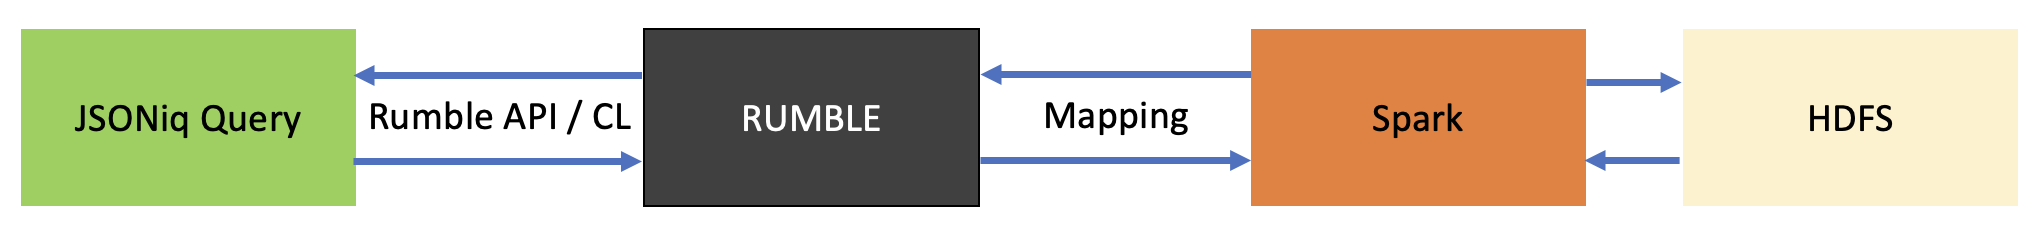
\includegraphics[width=\linewidth]{rumble_architecture.png}
	\caption{Rumble Architecture Overview}
	\label{fig:Rumble_Architecture}
\end{figure}

\subsection{Mapping}
\label{sec:RumbleMapping}
We said that Rumble has a logic that is capable of mapoing the query to Spark primitives. We also said that in JSONiq, everything is a Sequence of Items. Therefore, Rumble uses interface Item in the code \cite{RumbleRepository}. All 6 types mentioned in Section \ref{sec:JSON} implement this interface. After that, Item is wrapped using the Spark JavaRDD generic class and the mapping is complete. Spark is now able to execute queries using objects of the wrapper class.\todo{Maybe I should present the full inheritance tree with subtypes as well}

As also said, FLWOR Expressions are the most powerful ones and we can view them as a set of clauses. Between themselves, clauses operate by consuming tuple streams instead of operating on Sequence of Items. Sequence of Items is produced only in the end with the mandatory Return clause. Therefore, in the code \cite{RumbleRepository}, Rumble uses class FlworTuple for wrapping to the Spark Dataset generic class that is used for DataFrames. For each clause, we have a RuntimeTupleIterator and they all, with the exception of Return, have a reference to FlworTuple. More details in Subsection \ref{sec:Generator}.
\todo{Or maybe I should just delete the whole Mapping since I have it at the end}

\subsection{General Architecture}
\label{sec:RumbleArchitecture}
So far, we were referring to Rumble as an engine. Essentially it is a compiler implemented in Java, and as such, it follows basic Compiler Design principles. In order not to break the declarative property of JSONiq query language, it requires proper separation of concerns. Irimescu in his thesis \cite{RumbleThesis} proposed the layered architecture described in Figure \ref{fig:Rumble_General_Architecture}. It consists of 4 main phases:
\begin{enumerate}
	\item Lexer and Parser take JSONiq query as an input and produce Abstract Syntax Tree - AST as the output 
	\item Translator takes the AST as the input and produces a tree of expressions - Expression Tree as the output
	\item Generator takes Expression Tree as input and converts it into a tree of runtime iterators - Runtime Iterator Tree
	\item Runtime iterators represent the code that can be executed on a single node or on top of Spark
\end{enumerate} 

\begin{figure}[h!]
	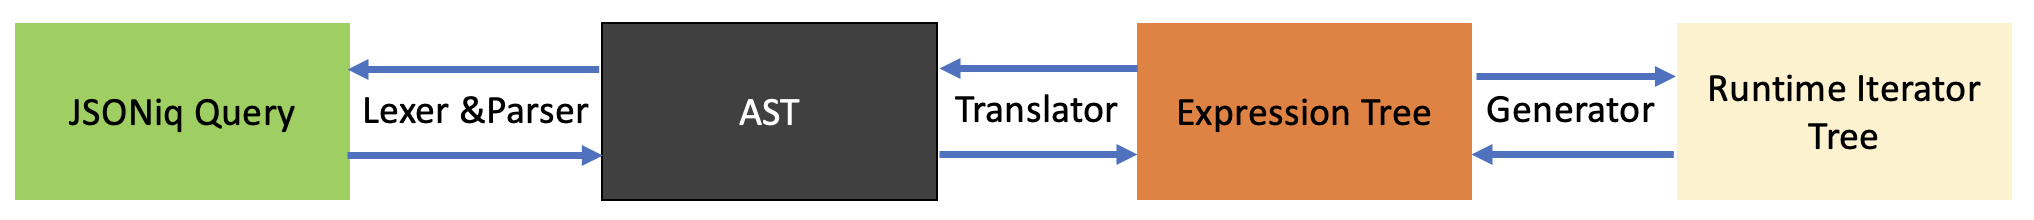
\includegraphics[width=\linewidth]{parsing_architecture.png}
	\vspace*{-5mm}
	\caption{Rumble General Architecture}
	\label{fig:Rumble_General_Architecture}
\end{figure}

\subsubsection{Lexer and Parser}
\label{sec:RumbleLexerParser}
The first steps in analyzing source code, in this case query written in JSONiq query language, are Lexical and Syntax analysis's performed by Lexer and Parser modules respectively. For rather simple languages, such as JSONiq, these two modules can be automatically generated from language grammar. Thus, Another Tool for Language Recognition - ANTLR v4 framework \cite{ANTLR} is used. ANTLR needs a grammar (.g4) file with definitions of all language constructs as the input. For Rumble, JSONiq.g4 file was implemented and using it ANTLR auto-generated Parser and Lexer together with BaseVisitor (implements visitor pattern) Java classes. In the code, you can first use the Lexer class that takes JSONiq query stream as input and then pass it to Parser class which will generate AST and conclude the so called "front-end" part of compiler.

\subsubsection{Translator}
In general with compilers, AST cannot be used directly. As explained in \cite{RumbleMLThesis}, JSONiq is a functional language that is composed of expressions. Thus, higher-level abstractions - Expression Tree is needed. To achieve higher-level abstractions, the following classes had to be implemented. On top of the inheritance tree, we have abstract class Node from which Expression and Clause classes are derived. Clause class is then used for deriving all clauses of FLWOR Expression. For all other Expression types mentioned in Section \ref{sec:JSONiq}, classes were derived from the Expression class. 

The second part of generating the Expression Tree required specific implementation of BaseVisitor class generated by ANTLR. BaseVisitor is a generic class and its specific implementation - TranslationVisitor class wraps around Node class. 

The third part of generating the Expression Tree is the Static Context class containing a map between variable names and sequence types. Each Expression has its own Static Context.

Using all these classes, it is then possible to generate th Expression Tree as explained in \cite{RumbleThesis}: 

"The visitor starts at the top-level Expression and then moves through all of the children passing along the current Static Context while doing three things:
\begin{enumerate}
	\item For any expression that it visits, it sets the Static Context to be equal to the currently generated one.
	\item For any variable reference, it checks that the variable name is present in the current Static Context, otherwise it throws an error (at compile time).
	\item For any variable declaration it creates a new Static Context containing the new variable and sets the previously existing Static Context as parent."
\end{enumerate}

\subsubsection{Generator}
\label{sec:Generator}
So-called "back-end" - the last part of compiler includes code generation where the intermediate code gets transformed into assembly instruction and finally machine instructions. For this step in Rumble, we are performing conversion from Expression Tree to a tree of runtime iterators. As Rumble was written in Java, runtime iterators are in charge of executing operations that get converted to Java bytecode.

All RuntimeTupleIterator implement RuntimeTupleIteratorInterface while all other runtime iterators implement RuntimeIteratorInterface. Both interfaces are similar to java.util.Iterator interface with methods such as hasNext() and next(). Using next(), runtime iterators can iterate over Sequence of Items and return results one Item at a time. In addition, next() method triggers the computation of all children iterators by recursively calling next() method in them. Result of such implementation is "lazy evaluation", where results are computed only when demanded. 

These two runtime interfaces operate on Dynamic Context containing a map between variable names and actual sequences of items. Static Context is in charge of static type checking performed at compile-time, while Dynamic Context is in charge of dynamic type checking performed at runtime.

As pointed out in \cite{RumblePaper} "The main novelty in the design of Rumble is the runtime iterators that can switch dynamically between different execution modes, and which encode the decision of which nesting level is distributed." In total, there are 3 different execution modes. In local execution mode runtime iterators are executed on a single node locally in Java and they do not push computation to Spark. The other two, RDD-based execution (which uses Spark’s RDD interface) and  DataFrame-based execution (which uses the DataFrame interface), are executed on top of Spark. They both push computation to spark when a dataset is large and there is a clear advantage over local execution mode. The modes that a runtime iterator supports are based on JSONiq Expression category and presented in Table \ref{tab:RuntimeCategoriesMapping}. The column "As in JSONiq" represents classification as we have seen it before in Section \ref{sec:JSONiq} where Built-in Function and Sequence Construction are omitted since they are spread across several categories. The columns L, R and D represent local, RDD-based and DataFrame-based execution modes, respectively, while + signifies that this mode is supported.

\begin{table}[h!]
		\vspace{-1mm}
	\centering
	\resizebox{\textwidth}{!}{%
	\begin{tabular}{|l|l|l|l|l|l|} 
		\hline
		\textbf{Category}                      & \textbf{Expression/Clause}                                  & \textbf{As in JSONiq~}                                                                                                   & \textbf{L}         & \textbf{R}         & \textbf{D}          \\ 
		\hline
		\multirow{5}{*}{local-only}            & (),~\{\$k:\$v\},~[\$seq],~\$\$,~+,~-,~mod,~                 & \multirow{5}{*}{\begin{tabular}[c]{@{}l@{}}Arithmetic,\\Comparison,\\Logic,\\Literal,\\JSON construction\end{tabular}} & \multirow{5}{*}{+} & \multirow{5}{*}{}  & \multirow{5}{*}{}   \\ 
		\cline{2-2}
		& div,~idiv,~eq,~ne,~gt,~lt,~ge,~le,~and,~                    &                                                                                                                        &                    &                    &                     \\ 
		\cline{2-2}
		& or,~not,~\$a\textbar{}\textbar{}\$b,~\$f(\$x),~\$m~to~\$n,~ &                                                                                                                        &                    &                    &                     \\ 
		\cline{2-2}
		& try catch, instance~of, castable,                           &                                                                                                                        &                    &                    &                     \\ 
		\cline{2-2}
		& cast, some~\$x~in~\$y~satisfies...                          &                                                                                                                        &                    &                    &                     \\ 
		\hline
		\multirow{2}{*}{sequence-transforming} & \$seq[...],~\$a[\$i],~\$a[],~\$a[[]],~\$o.\$s,              & \multirow{2}{*}{JSON navigation}                                                                                       & \multirow{2}{*}{+} & \multirow{2}{*}{+} & \multirow{2}{*}{+}  \\ 
		\cline{2-2}
		& \$seq!..., annotate, treat                                  &                                                                                                                        &                    &                    &                     \\ 
		\hline
		\multirow{3}{*}{sequence-producing}    & json-file, parquet-file, libsvm-file,~                      & \multirow{3}{*}{}                                                                                                      & \multirow{3}{*}{}  & \multirow{3}{*}{+} & \multirow{3}{*}{+}  \\ 
		\cline{2-2}
		& text-file, csv-file,~avro-file, root- file,                 &                                                                                                                        &                    &                    &                     \\ 
		\cline{2-2}
		& structured-json-file, parallelize                           &                                                                                                                        &                    &                    &                     \\ 
		\hline
		\multirow{3}{*}{sequence-combining}    & seq1,\$seq2, if (\$c) then... else...,                      & \multirow{3}{*}{}                                                                                                      & \multirow{3}{*}{+} & \multirow{3}{*}{+} & \multirow{3}{*}{+}  \\ 
		\cline{2-2}
		& switch (\$x) case... default...,                            &                                                                                                                        &                    &                    &                     \\ 
		\cline{2-2}
		& typeswitch (\$x) case... default...                         &                                                                                                                        &                    &                    &                     \\ 
		\hline
		\multirow{2}{*}{FLWOR}                 & for,~let,~where,~group~by,~                                 & \multirow{2}{*}{FLWOR}                                                                                                 & \multirow{2}{*}{+} & \multirow{2}{*}{}  & \multirow{2}{*}{+}  \\ 
		\cline{2-2}
		& order~by,~count, return                                     &                                                                                                                        &                    &                    &                     \\
		\hline
	\end{tabular}}
	\caption{Runtime iterator categorization for JSONiq expressions and clauses}
	\label{tab:RuntimeCategoriesMapping}
	\vspace{-3mm}
\end{table}

\todo{Check if table makes sense for the plus signs because at the end of this section we have additional explanation which primitives are used (RDD union, flatmap etc...)}
Local-only iterators executed in the local execution mode come down to implementing the Expression's behavior in Java. On the other hand, RDD and DataFrame-based execution modes require a mapping to Spark primitives as explained in Section \ref{sec:RumbleMapping}. There is an essential difference between these two modes that are running on top of Spark. The DataFrame-based mode is used in the case that internal structure is known statically. This mode is also preferred over RDD-based mode as it faster in execution. On the other hand, the RDD-based mode is used whenever the structure is unknown. 

Rumble, in its initial version, was using RDD-based mode for FLWOR Expressions. However, all FLWOR Clauses Iterators, with the exception of Return, operate with FlworTuple. From the query, it is possible to derive the static type of the variables in the tuples and therefore represent them as columns in DataFrame. Today, the RuntimeTupleIterator is using SQL queries instead of RDD transformations of Spark. We will not explain the new mappings for each and every FLWOR Clause in detail, but we will make a parallel to For Clause and reuse an example from \cite{RumblePaper}. If the current variables are x, y, and z, and the new variable introduced by the for clause is i, then the for clause is mapped to the following:

SELECT x, y, z, EXPLODE(UDF(x, y, z)) AS i FROM input\_stream

Spark’s EXPLODE functionality corresponds to flatMap() on RDDs, while UDF is a Spark SQL user-defined function that takes all existing variables as input, and returns the resulting sequence of items as a List$<$Item$>$.

%Regarding all sequence category of runtime iterators, they all operate on sequences of items. Since item is essentially an interface and we have a polymorphic class hierarchy as all 6 JSON types implement it, we cannot use Dataframes but we use RDDs instead. Therefore, Sequence-transforming Expressions are handled using map(), flatMap(), and filter() transformations in Spark. Sequence-combining Expressions use RDD.union. There is a small exception for Sequence-producing Expressions. Only for json-file() and text-file() the structure is unknown, for all other file formats, structure is known and therefore Dataframe can be used. 
\chapter{XQuery/XPath 3.* Test Suite(QT3TS)}
\section{Analysis}
In this chapter, we will discuss design decisions that we have made during the development of Test Driver. The core idea is to develop Test Driver completely independently from Rumble by maintaining the code outside of Rumble.

\subsection{Programming Language}
 We view Rumble as black-box and the single point of communication with Rumble should only be via the Rumble Java public API. Therefore, we have decided to implement Test Driver as Java Console Application. Furthermore, Rumble is also written in Java. We decided to setup our Java Console Application project to have two modules - Test Driver and Rumble module. Rumble module is the branch in repository created for the purpose of this work \cite{RumbleBranch}. Making Test Driver module dependent on it, we are allowing possibility to directly use Rumble and its classes in case that not everything is possible to be achieved by treating Rumble as the black-box. 

\subsection{Data Format}
The XQuery/XPath 3.* Test Suite (QT3TS) is publicly available at W3C Public CVS Repository under module name 2011/QT3-test-suite \cite{TestSuiteCVSRepository}. Since April 1st 2019, CVS tree has been discontinued and the repository has been migrated to W3C Public GitHub repository \cite{TestSuiteGitHubRepository}. The tests are published as a set of files - test sets containing in total more than 30000 test cases. The tests are published as a set of files, mostly in XML format. W3C does not supply a Test Driver for executing the tests. Instead, for each implementation a Test Driver should be written. As these test sets are mostly written in XML format, the first component that our Test Driver will require is the XML parser. 

\subsection{XML Parser}
XML parser is a program that allows our application to read and write XML documents. For our work, we have investigated following possibilities:
\begin{itemize}
	\item DOM (Document Object Model) - This parser loads entire XML document in memory and uses interfaces to access the information. It can access couple of item elements at same time. It can be used for both reading and writing.
	\item SAX (Simple API for XML parsing) - This parser doesn't load XML document in memory. Instead, it allows us to register a handler with SAX parser. When parser goes through file it keeps invoking methods on the handler class for each item. It process it in sequence one at a time. For each new item it reads, it forgets state of previous items. Therefore, on each read we need to take appropriate action in our application. It is read only and also known as push parser. There is no handler on XML document side, only in our application.
	\item STAX (Streaming API for XML parsing) - This parser allows us to both read and write multiple documents at same time. Unlike SAX that reads one item at a time, STAX can be explicitly asked to get a certain item from XML document without loading it in memory. Therefore, we can look at it as mixture of DOM and SAX. It is pull parser and has handler on XML document as well
	\item JAXP (JAVA API for XML parsing) - Since JDK 1.5, the JAXP API has been available as a standard part of the Java platform, and it provides access to XSLT transformation, schema validation, and XPath processing services.
	\item Saxon \cite{Saxon} - Open Source XSLT \& XQuery processor developed by Saxonica Limited. The Saxon package is a collection of tools for processing XML documents. The main components accessible via API are:
	\begin{enumerate}
		\item XSLT processor. Saxon implements the XSLT 3.0 Recommendation. The product can also be used to run XSLT 2.0 stylesheets, or XSLT 1.0 stylesheets in backwards compatibility mode.
		\item XPath processor. This supports XPath 2.0 and XPath 3.1. It can also be used in backwards-compatibility mode to evaluate XPath 1.0 expressions.
		\item XQuery processor. This supports XQuery 3.1, which also allows XQuery 1.0 or 3.0 queries to be executed. 
		\item XML Schema Processor. This supports both XSD 1.0 and XSD 1.1. It can be used to support the schema-aware functionality of the XSLT and XQuery processors.
	\end{enumerate}
\end{itemize}

For parsing XML, we have decided to use Saxon. One may argue that for all 4 listed components, Java also has its own API – JAXP for 1st, 2nd and 4th together with XQJ for 3rd. However, in practice, Saxon is easier to use and more flexible than JAXP. Apart from that, main arguments are:
\begin{enumerate}
	\item Saxon itself is one of the implementations for which Test Driver was also implemented. Based on Results Report \cite{SaxonReport}, it passes more than 99,9\% of the QT3TS tests.
	\item Saxons implementation of the Test Driver can be used as a baseline for developing our own Test Driver. 
\end{enumerate}

\section{Phase 1 Implementation}
\subsection{Description}
\label{Phase1_Description}
In the first phase of the implementation we have analyzed the structure of QT3TS. We had to understand the under-laying structure of each and every test case. We had to see under which tags the information is stored in order to obtain it using Saxon API. Example test case in XML format:

\lstinputlisting{source_code_1.xml}

The two most important tags in each test case are:
\begin{itemize}
	\item Test  - this is the test that should be executed on Rumble. It can be XSLT, XPath or XQuery expression.
	\item Result - this is the expected result outcome of the test tag. As it can be seen in the provided example, there are several types of assertions that we need to verify.
\end{itemize}

Test Driver's Test Case Handling Logic is supposed to iterate over catalog.xml using the Saxon API. This XML document contains list of all test-sets. Again, using the Saxon API, we iterate over test-cases in each of the test-sets. For each test-case, we are asking explicitly Saxon XML parser to get items under Test and Result tags. To use Saxon API, we need to know the structure. But, once Test Case Handling Logic obtains information under Test tag, it passes it down "as is" to Rumble API in order to execute the query. Rumble API returns the result which is then passed down to Test Result Handling Logic. 

Test Driver's Test Result Handling Logic is in charge of determining which assertion needs to be performed. Here we provide the list of possible assertions:

\begin{itemize}
	\item assert-empty - This assertion requires result to return empty sequence
	\item assert - This assertion requires us to run another query in which obtained result will be used as parameter of the new query. For example:
	\lstinputlisting{source_code_2.xml}
	\item assert-eq - It requires us to run another query in form of obtained result "eq" value under the assert-eq tag
	\item assert-deep-eq - Similar to assert-eq but runs "deep-equal" query
	\item assert-true - It requires result to return single Boolean value True
	\item assert-false - Opposite of assert-true
	\item assert-string-value - It requires that each item in the obtained result sequence is type of String and also "eq" to the sequence under this tag
	\item all-of - It contains multiple different assert tags described in this list and it requires all of them to be fulfilled 
	\item any-of - Similar to all-of but requires only one of them to be fulfilled
	\item assert-type - Requires to check if obtained result is instance of this tag
	\item assert-count - It requires obtained result sequence size to be equal to the value under assert-count tag
	\item not - It requires to execute nested assertion with a negation
\end{itemize}

After the assertion is performed, we need to classify the results. The idea is to make statistics that are described in \ref{Phase1_Results}. With such a classification we would be able to improve Rumble by reporting bugs in its implementation.

\subsection{Architecture}
The overview of scenario described in \ref{Phase1_Description} can be seen in Figure \ref{fig:Phase1_Architecture}
 \begin{figure}[h!]
 	\vspace*{-5mm}
 	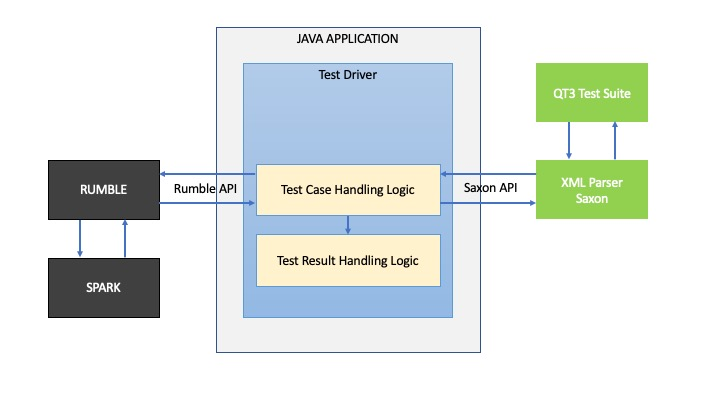
\includegraphics[width=\linewidth]{architecture_diagram_phase_1.jpeg}
 	\vspace*{-15mm}
 	\caption{Phase 1 Architecture Overview}
 	\label{fig:Phase1_Architecture}
 \end{figure}
 
\subsection{Results}

\label{Phase1_Results}
As explained in \ref{Phase1_Description}, result obtained via Rumble API was compared with the expected result by applying the correct assertion check. In case assertion passed, test-case was considered a Success and otherwise Fail. The block of code performing these operations was surrounded by try and catch. In case that test failed because the syntax was not completely JSONiq, it would throw a RumbleException or more generally an Exception - Crash. With this implementation, we were to be able to distinguish 3 possible scenarios:

\begin{enumerate}
	\item Success - Test case succeed
	\item Fail - Test case failed because of bug in Rumble
	\item Crash - Test case failed because it is not compatible with Rumble
\end{enumerate}

The report is generated as .csv file having test-sets as rows and total number of test-cases per scenario in the columns. In Table \ref{tab:Phase1_ResultTable} we will present the aggregated sum over all rows in the .csv file:

\begin{table}[h!]
	\centering
	\begin{tabular}{|l|r|r|}
		\hline
		\multicolumn{1}{|c|}{Scenario} & \multicolumn{1}{c|}{Total test-cases} & \multicolumn{1}{c|}{\% of all test-cases} \\ \hline
		Success                        & 2330                                  & 7.8                                       \\ \hline
		Fail                           & 2769                                  & 8.8                                       \\ \hline
		Crash                          & 26421                                 & 83.4                                      \\ \hline
	\end{tabular}
 	\caption{Phase 1 Results Overview}
 	\label{tab:Phase1_ResultTable}
\end{table}

\section{Phase 2 Implementation}
\subsection{Description}
\label{Phase2_Description}
After generating Phase 1 Implementation report described in Table \ref{tab:Phase1_ResultTable}, we carefully examined our implementation and identified 4 major pain points:
\begin{itemize}
	\item Unstable implementation of assertion which resulted in implementing proper way of result binding in Rumble
	\item Too many crashing tests which resulted in implementing converter
	\item Insufficient granularity for distinguishing test-cases
	\item Improving Test Driver implementation resulted in breaking previously implemented features. Therefore, regression tests were introduced
\end{itemize}

\subsubsection{Result Binding}
To better understand the issues we have encountered, we will provide following code snippet:
\lstinputlisting{source_code_without_results.java}

If we examine the AssertEq implementation, we will notice that lines.get(0) assumes that obtained result is a single item and takes first one. It does not handle sequences! Furthermore, handling sequences was only possible for AssertStringEqual in case that our result is sequence of strings by performing string concatenation. All other assertions such as Assert, AssertEq, AssertDeepEq are not possible to be implemented. Finally, if we remember Assert example from Section \ref{Phase1_Description}, we will notice that we had to perform string replace of \$result with actual result obtained from the Rumble API. 

Thus, Rumble was extended to support result binding. The change was made in Rumble implementation itself. The only modification required in Test Driver was to instantiate a new RumbleConfiguration and also new Rumble instance for each test-case that requires result binding. Check code below:

\lstinputlisting{source_code_with_results.java}

The main concern of the new implementation was that performing many instantiates might cause the execution time to increase dramatically. However, after run-time increased only by 15seconds from 2minutes - only 12.5\%.

Once the result binding was implemented, it allowed us to run the assert type also as a query instead of calling the publicly exposed methods of the Item class in the Rumble Java API. In Phase 1 implementation, we had a switch case for every possible type that Rumble Java API supports, making code difficult for future maintenance and extension with new supported types. With running assert type as "instance of" query , we managed to have a single point of conversion performed in the beginning and applied for both test case and the expected result. Within conversion we would discover the unsupported type errors without the need of second switch case to check whether Rumble's API Item class supports the type or not. Furthermore, the previously implemented switch case had unsupported type as default therefore hiding some types that were supported but not specified in the documentation. The mentioned conversion will be explained more in detail in Section \ref{Phase2_Converter}. 

The clean separation that was performed here initialized idea and was a base plan for XQuery to JSONiq conversion logic separation. In Section \ref{Phase3_Description} we will describe Architecture that has separate application that takes XQuery as input, performs conversion and outputs JSONiq test suite. Such approach would make the Test Driver easily maintainable and extensible!

\subsubsection{Converter}
\label{Phase2_Converter}
As seen in Table \ref{tab:Phase1_ResultTable}, we had less than 10\% Success test-cases as almost all of them required conversion to JSONiq. Here we will document all the conversions that we have performed on both Test and Result tags in this Phase. 

The first conversion that we have performed is between types. Both XQuery and JSONiq have simple(atomic) and complex(non-atomic) types. 

The list of atomic types that is currently supported by Rumble was taken from official Rumble documentation \cite{RumbleSupportedTypes} and conversion was implemented accordingly. For all types that are not supported, our code throws UnsupportedTypeException. 

Following 3 complex (non-atomic) types were handled by following conversion:
\begin{enumerate}
	\item array(*) was replaced with array*
	\item item() was replaced with item
	\item map(string, atomic) was replaced with object 
\end{enumerate}

On the other hand, following 7 complex (non-atomic) types could not be converted and they all throw UnsupportedTypeException:
\begin{enumerate}
	\item document
	\item element
	\item attribute
	\item text
	\item comment
	\item processing-instruction
	\item xs:QName
\end{enumerate}

Other conversions that were performed:
\begin{enumerate}
	\item true() was replaced with true
	\item false() was replaced with false
	\item INF was replaced with Infinity
	\item array access via . was replaced with \$\$
	\item ' was replaced with "
	\item prefixes fn, math, map, array were removed
\end{enumerate}

Other items that were unsupported in Phase 2 were node(), empty-sequence() and xs:NOTATION together with all error codes that are not in Table \ref{tab:Phase2_Supported Types} that was taken from \cite{RumbleSupportedErrorCodes}.

\subsubsection{Regression Tests}
During Phase 1, we were performing iterations with goal to overall improve Test Driver's implementation. The good metric while performing these iterations was total number of test-case Crashes. Our goal was to reduce those numbers as much as possible. This was mainly handled by making following changes: bug fixes, software enhancements, configuration changes. Creating this changes in software development can usually lead to creating new issues that were not present before or re-emergence of old issues. In these cases it is quite common that software development requires regression testing.
\todo{MAYBE CITE SOMETHING} Regression testing (rarely non-regression testing[1]) is re-running functional and non-functional tests to ensure that previously developed and tested software still performs after a change.[2] If not, that would be called a regression. 
\todo{Copied from Wikipedia}. During iterations, it was noticed that our approach of fixing and improving the application is highly exposed to changes that require regression testing. 

While performing iterations, we had to ensure that any further implementation would not break the test-cases that were passing before and at the same time not introduce new test-cases that are Crashing. Thus, for each iteration we have maintained log files of all Passed (Success + Managed) and Crashed test-cases. In every next iteration we have done two comparison between new and previous log files. We have performed a check that compared whether all the passed test-cases from the previous implementation were also contained in the new implementation or not and created "List of test cases that were passing before but not anymore". For Crashes, we did opposite check and created list of "Tests that were not crashing before, but are now and not in list above". 

\subsection{Architecture}
\todo{Maybe the Exceptions arhictecutre here as well}
The overview of scenario described in \ref{Phase2_Description} can be seen in Figure \ref{fig:Phase2_Architecture}
\begin{figure}[h!]
	\vspace*{-5mm}
	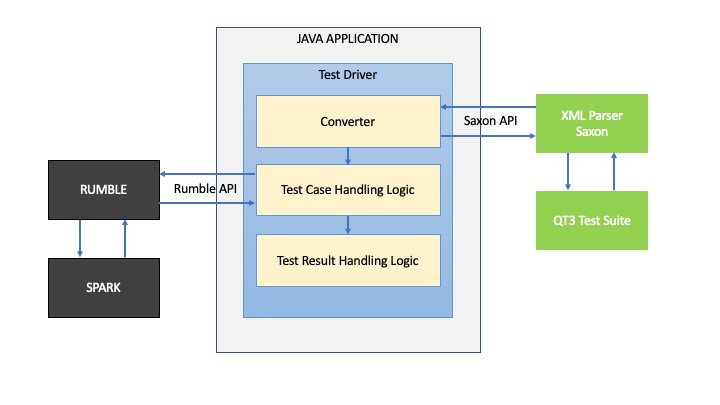
\includegraphics[width=\linewidth]{architecture_diagram_phase_2.jpg}
	\vspace*{-15mm}
	\caption{Phase 1 Architecture Overview}
	\label{fig:Phase2_Architecture}
\end{figure}

\subsection{Results}
As we have seen in Section \ref{Phase2_Converter}, Crashes were not only capturing tests that are not JSONiq and needed conversion. They were also including the tests that could not succeed simply because Rumble does not support that feature, type or error code. In Table \ref{tab:Phase2_Supported Types} we can see the limited amount of supported types and error codes compared to XQuery w3 specification for which we are able to verify assertion. All others would then be ignored and classified differently. Furthermore, some of them were introducing dependencies. For example, in dependency tag it was possible to have request for particular version of XPath, XQuery or XSLT. While Rumble is backwards compatible with all versions of XPath and XQuery, it does not support XSLT. We have therefore created and divided test cases into 7 groups:
\begin{enumerate}
	\item Success – Test that is passing the assertion and does not need Converter
	\item Managed – Tests that would have failed assertion, but they were modified with hard-coded conversion into JSONiq using Converter
	\item Skipped – Test that is not JSONiq and thus expectedly fails assertion. These tests should not be converted to JSONiq
	\item Failed – Tests that are failing because there is a bug in Rumble API or Test Driver implementation. 
	\item Dependency – Tests that are failing because dependency is not supported
	\item Unsupported – Tests that are failing because type, feature or error code is not supported yet
	\item Crash – Any other exception
\end{enumerate}

After introduction of the 7 above mentioned cases, together with small adjustments and bug changes, we were able to obtain:
\begin{table}[h!]
	\centering
	\begin{tabular}{|l|r|r|}
		\hline
		\multicolumn{1}{|c|}{Scenario} & \multicolumn{1}{c|}{Total test-cases} & \multicolumn{1}{c|}{\% of all test-cases} \\ \hline
		Success                        & 2686                                  & 8.52                                      \\ \hline
		Managed                        & 4211                                  & 13.36                                     \\ \hline
		Fail                           & 2554                                  & 8.10                                      \\ \hline
		Skipped                        & 5                                     & 0.02                                      \\ \hline
		Dependency                     & 1481                                  & 4.70                                      \\ \hline
		Crash                          & 13171                                 & 41.79                                     \\ \hline
		Unsupported                    & 7412                                  & 23.52                                     \\ \hline
	\end{tabular}
	\caption{Phase 2 Results Overview}
	\label{tab:Phase2_ResultTable}
\end{table}

Managed category was introduced as it was identified that with simple hard-coded conversion we are able to obtain around 4200 passed tests increasing total percentage of passed tests by roughly 12\%. At first, it seems that Success and Managed should be grouped into single category, but we decided to keep them separated. The reason behind is that while fixing bugs in both Rumble and Test Driver, we will increase the number of Success test cases. At the same time, we want to keep the track of Managed ones, because in Phase 3 Implementation we are planning to generalize the hard-coded conversion and create pure JSONiq Test Suite based on given XML ones.

For Skipped tests, these are the ones that it would not make sense to try to convert them to JSONiq. One example is XSLT tests and those should be skipped. We are keeping them in separate list as in Phase 3 Implementation we will skip from output and not include them in pure JSONiq Test Suite.

The main goal of performing iterations was to go through all the crashes and try to completely eliminate them. By doing so we would also improve the statistics by classifying them into other categories. At the same time, we were manually investigating test cases and trying to find the root cause. For some of them, our Test Driver implementation was improved. For some it was identified that the XQuery function was not yet supported by Rumle or it was having bugs so Rumble implementation was also improved. List of dependencies that were found in Test Suite were documented and classified according to Rumble documentation. The list is presented in Table \ref{tab:Phase2_DependencyList} \todo{maybe some reference here, ask Fourny}. 

Final goal was to identify test-cases that fail but can be converted to JSONiq. They could not be included into the automatic distinction of 7 above mentioned cases and had to be handled manually. They also helped with identifying what Phase 3 conversion also had to support.

\section{Phase 3 implementation}
\subsection{Description}
\label{Phase3_Description}
The main issue of Converter described in Section \ref{Phase2_Converter} was that it was hard-coded conversion using Java String.replace method. Such implementation can be very unstable. For example, we can look at 5th item of "other conversions" mentioned in Section \ref{Phase2_Converter} - replacing ' with ". For example, test-case Literals009 is verifying whether "test' is a valid String Literal. With our hard-coded conversion, we will make this test-case valid String Literal instead of it causing an Error Code XPST0003. Therefore, we have decided to implement Test Converter as separate module. It's main purpose is to generalize the hard-coded conversion. It would take QT3TS as Input and generate pure JSONiq Test Suite as output.

For implementing Test Converter we decided to create following classification of test-cases:
\begin{enumerate}
	\item Fails, as expected and should not be converted to JSONiq. It will never be supported
	\item Fails, as expected since it is not supported yet
	\item Fails, but can be rescued with simple conversion. Any simple conversion like removing the "fn" prefix 
	\item Fails, but can be converted to JSONiq. Any complicated conversion like XML to JSON
	\item Fails, because it is bug in Rumble
	\item Succeeds
\end{enumerate}

With this classification, we want to reuse most of Phase 2 Implementation Results presented in Table \ref{tab:Phase2_ResultTable}.

If we compare above described classification with classification in Table \ref{tab:Phase2_ResultTable}, we can notice that Fail corresponds to Item 5. Item 6 corresponds to Success. Managed corresponds to Item 3. Item 2 corresponds to Unsupported and Dependency. Skipped correspond to Item 1. 

Performing iterations in Phase 1, we want to distribute all Crashes into some of Item 4 or 1. Of course, it is in our interest to identify as many test-cases as possible as Item 4 and perform conversion in Test Converter. Everything that we cannot convert, we will classify as Item 1. 

Items 1 will be excluded from Test Converter output. Items 2 on the other hand, will be excluded from Test Driver input. However, we also need to take into account that over time, as Rumble implementation improves, tests from Item 2 will be distributed into 4 other categories. Therefore, we want to make highly modular and extensible architecture. The important design decision remaining is the Data Format of the Test Converted output.

\subsubsection{JSONiq and Test Converter Data Format}
The JSONiq extension to XQuery allows processing XML and JSON natively and with a single language. This extension is based on the same data model as the core JSONiq and is based on the same logical concepts. Because of the complexity of the XQuery grammar, the JSONiq extension to XQuery has a less pleasant syntax that the JSONiq core. \todo{maybe cite something}. When designing the Test Converter, we could have decided to use either XML or JSON as the under-laying language. However, as our Test Driver was already implemented in the previous phase and was expecting XML as input and using the before mentioned Saxon for parsing it, we have decided to keep the same language for output of the Test Converter. 

\subsection{Architecture}
The overview of scenario described in \ref{Phase3_Description} can be seen in Figure \ref{fig:Phase3_Architecture}
\begin{figure}[h!]
	\vspace*{-5mm}
	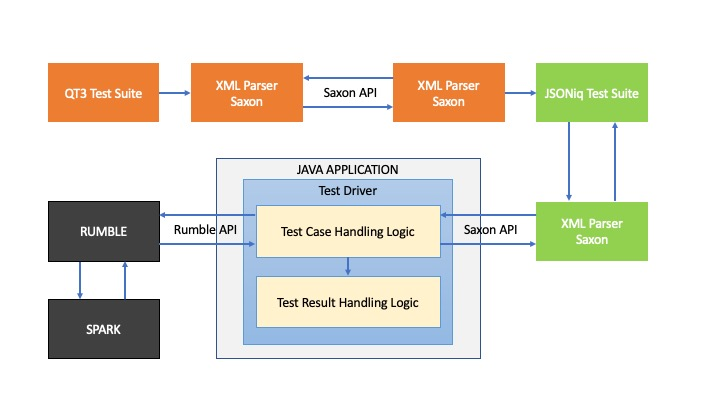
\includegraphics[width=\linewidth]{architecture_diagram_phase_3.jpg}
	\vspace*{-15mm}
	\caption{Phase 1 Architecture Overview}
	\label{fig:Phase3_Architecture}
\end{figure}

\subsection{Results}
After carefully analyzing the complete QT3TS, we have concluded that out of 424 test-sets QT3TS consists of, total of 143 can be classified of belonging in the Item 1 or Item 2 of classification documented in this phase of implementation. More specifically, we have assigned 61 test-sets to Item 1 presented in Table \ref{tab:Phase3_Item1} and 84 test-sets to Item 2 presented in Table \ref{tab:Phase3_Item2}.

In addition to test-sets assigned to Item 2, we are adding the Unsupported and Dependency. Furthermore, several bugs were fixed in Rumble between Phase 2 and Phase 3 Implementation resulting in:

\begin{table}[h!]
	\centering
	\begin{tabular}{|l|r|r|}
		\hline
		\multicolumn{1}{|c|}{Scenario} & \multicolumn{1}{c|}{Total test-cases} & \multicolumn{1}{c|}{\% of all test-cases} \\ \hline
		Item 1                         & 3675                                  & 11.65                                     \\ \hline
		Item 2                         & 12751                                 & 40.41                                     \\ \hline
		Item 3                         & 7007                                  & 22.20                                     \\ \hline
		Item 4                         & 4424                                  & 14.02                                     \\ \hline
		Item 5                         & 999                                   & 3.17                                      \\ \hline
		Item 6                         & 2701                                  & 8.56                                      \\ \hline
	\end{tabular}
	\caption{Phase 3 Results Overview}
	\label{tab:Phase3_ResultTable}
\end{table}


\begin{table}[]
	\begin{tabular}{lllr}
		\textbf{Type}      & \textbf{Status} &  & \multicolumn{1}{c}{\textbf{Supported Error Codes}} \\
		atomic             & supported       &  & FOAR0001                                           \\
		anyURI             & supported       &  & FOCA0002                                           \\
		base64Binary       & supported       &  & FODC0002                                           \\
		boolean            & supported       &  & FOFD1340                                           \\
		byte               & not supported   &  & FOFD1350                                           \\
		date               & supported       &  & JNDY0003                                           \\
		dateTime           & supported       &  & JNTY0004                                           \\
		dateTimeStamp      & not supported   &  & JNTY0024                                           \\
		dayTimeDuration    & supported       &  & JNTY0018                                           \\
		decimal            & supported       &  & RBDY0005                                           \\
		double             & supported       &  & RBML0001                                           \\
		duration           & supported       &  & RBML0002                                           \\
		float              & not supported   &  & RBML0003                                           \\
		gDay               & not supported   &  & RBML0004                                           \\
		gMonth             & not supported   &  & RBML0005                                           \\
		gYear              & not supported   &  & RBST0001                                           \\
		gYearMonth         & not supported   &  & RBST0002                                           \\
		hexBinary          & supported       &  & RBST0003                                           \\
		int                & not supported   &  & RBST0004                                           \\
		integer            & supported       &  & SENR0001                                           \\
		long               & not supported   &  & XPDY0002                                           \\
		negativeInteger    & not supported   &  & XPDY0050                                           \\
		nonPositiveInteger & not supported   &  & XPDY0130                                           \\
		nonNegativeInteger & not supported   &  & XPST0003                                           \\
		positiveInteger    & not supported   &  & XPST0008                                           \\
		short              & not supported   &  & XPST0017                                           \\
		string             & supported       &  & XPST0080                                           \\
		time               & supported       &  & XPST0081                                           \\
		unsignedByte       & not supported   &  & XPTY0004                                           \\
		unsignedInt        & not supported   &  & XQDY0054                                           \\
		unsignedLong       & not supported   &  & XQST0016                                           \\
		unsignedShort      & not supported   &  & XQST0031                                           \\
		yearMonthDuration  & supported       &  & XQST0033                                           \\
		&                 &  & XQST0034                                           \\
		&                 &  & XQST0038                                           \\
		&                 &  & XQST0039                                           \\
		&                 &  & XQST0047                                           \\
		&                 &  & XQST0048                                           \\
		&                 &  & XQST0049                                           \\
		&                 &  & XQST0052                                           \\
		&                 &  & XQST0059                                           \\
		&                 &  & XQST0069                                           \\
		&                 &  & XQST0088                                           \\
		&                 &  & XQST0089                                           \\
		&                 &  & XQST0094                                          
	\end{tabular}
	\caption{Rumble Supported Types and Error Codes}
	\label{tab:Phase2_Supported Types}
\end{table}

\begin{table}[]
	\begin{tabular}{ll}
		\textbf{Dependency name}           & \textbf{Status}              \\
		higherOrderFunctions               & supported                    \\
		moduleImport                       & supported                    \\
		arbitraryPrecisionDecimal          & supported                    \\
		schemaValidation                   & not supported (XML specific) \\
		schemaImport                       & not supported (XML specific) \\
		advanced-uca-fallback              & not supported                \\
		non\_empty\_sequence\_collection   & not supported yet            \\
		collection-stability               & not supported yet            \\
		directory-as-collection-uri        & not supported yet            \\
		non\_unicode\_codepoint\_collation & not supported                \\
		staticTyping                       & not supported yet            \\
		simple-uca-fallback                & not supported                \\
		olson-timezone                     & not supported yet            \\
		fn-format-integer-CLDR             & not supported yet            \\
		xpath-1.0-compatibility            & not supported (XML specific) \\
		fn-load-xquery-module              & not supported yet            \\
		fn-transform-XSLT                  & not supported yet            \\
		namespace-axis                     & not supported (XML specific) \\
		infoset-dtd                        & not supported (XML specific) \\
		serialization                      & not supported yet            \\
		fn-transform-XSLT30                & not supported yet            \\
		remote\_http                       & not supported                \\
		typedData                          & not supported                \\
		schema-location-hint               & not supported (XML specific) \\
		calendar                           & not supported yet            \\
		unicode-version                    & supported                    \\
		unicode-normalization-form         & supported                    \\
		format-integer-sequence            & not supported yet            \\
		xsd-version                        & supported                    \\
		xml-version                        & supported                    \\
		default-language                   & only "en" supported          \\
		language                           & only "en" supported          \\
		spec                               & only "XT30+" not supported   \\
		limits                             & not supported yet           
	\end{tabular}
	\caption{Supported Dependency List }
	\label{tab:Phase2_DependencyList}
\end{table}

\begin{table}[]
	\centering
	\begin{tabular}{ll}
		fn/base-uri.xml                                                                 & prod/AxisStep.ancestor-or-self.xml                                                  \\
		fn/doc.xml                                                                      & prod/AxisStep.following.xml                                                         \\
		fn/document-uri.xml                                                             & prod/AxisStep.following-sibling.xml                                                 \\
		fn/element-with-id.xml                                                          & prod/AxisStep.preceding.xml                                                         \\
		fn/generate-id.xml                                                              & prod/AxisStep.preceding-sibling.xml                                                 \\
		fn/has-children.xml                                                             & prod/AxisStep.static-typing.xml                                                     \\
		fn/id.xml                                                                       & prod/AxisStep.unabbr.xml                                                            \\
		fn/idref.xml                                                                    & prod/BoundarySpaceDecl.xml                                                          \\
		fn/innermost.xml                                                                & prod/CompAttrConstructor.xml                                                        \\
		fn/in-scope-prefixes.xml                                                        & prod/CompDocConstructor.xml                                                         \\
		fn/json-to-xml.xml                                                              & prod/CompCommentConstructor.xml                                                     \\
		fn/lang.xml                                                                     & prod/CompElemConstructor.xml                                                        \\
		fn/name.xml                                                                     & prod/CompNamespaceConstructor.xml                                                   \\
		fn/namespace-uri.xml                                                            & prod/CompPIConstructor.xml                                                          \\
		fn/namespace-uri-for-prefix.xml                                                 & prod/CompTextConstructor.xml                                                        \\
		fn/nilled.xml                                                                   & prod/ConstructionDecl.xml                                                           \\
		fn/node-name.xml                                                                & prod/ConstructionDecl.schema.xml                                                    \\
		fn/outermost.xml                                                                & prod/Comment.xml                                                                    \\
		fn/parse-xml.xml                                                                & prod/CopyNamespacesDecl.xml                                                         \\
		fn/parse-xml-fragment.xml                                                       & prod/DirAttributeList.xml                                                           \\
		fn/path.xml                                                                     & prod/DirectConstructor.xml                                                          \\
		fn/resolve-QName.xml                                                            & prod/DirElemConstructor.xml                                                         \\
		fn/root.xml                                                                     & prod/DirElemContent.xml                                                             \\
		fn/xml-to-json.xml                                                              & prod/DirElemContent.namespace.xml                                                   \\
		xs/token.xml                                                                    & prod/DirElemContent.whitespace.xml                                                  \\
		op/except.xml                                                                   & prod/NameTest.xml                                                                   \\
		op/intersect.xml                                                                & prod/NodeTest.xml                                                                   \\
		op/is-same-node.xml                                                             & prod/SchemaImport.xml                                                               \\
		prod/AxisStep.xml                                                               & prod/StepExpr.xml                                                                   \\
		prod/AxisStep.abbr.xml                                                          & prod/ValidateExpr.xml                                                               \\
		prod/AxisStep.ancestor.xml                                                      &                                                                                    
	\end{tabular}
	\caption{Item 1 - Fails, as expected and should not be converted to JSONiq. It will never be supported}
	\label{tab:Phase3_Item1}
\end{table}

\begin{table}[]
	\centering
	\begin{tabular}{ll}
		fn/compare.xml                            & map/size.xml                               \\
		fn/analyze-string.xml                     & map/put.xml                                \\
		fn/collation-key.xml                      & map/remove.xml                             \\
		fn/contains-token.xml                     & map/for-each.xml                           \\
		fn/data.xml                               & array/append.xml                           \\
		fn/default-collation.xml                  & array/filter.xml                           \\
		fn/default-language.xml                   & array/fold-left.xml                        \\
		fn/environment-variable.xml               & array/fold-right.xml                       \\
		fn/escape-html-uri.xml                    & array/for-each.xml                         \\
		fn/filter.xml                             & array/for-each-pair.xml                    \\
		fn/fold-left.xml                          & array/get.xml                              \\
		fn/fold-right.xml                         & array/head.xml                             \\
		fn/for-each.xml                           & array/insert-before.xml                    \\
		fn/for-each-pair.xml                      & array/join.xml                             \\
		fn/format-integer.xml                     & array/put.xml                              \\
		fn/format-number.xml                      & array/remove.xml                           \\
		fn/function-lookup.xml                    & array/reverse.xml                          \\
		fn/function-arity.xml                     & array/sort.xml                             \\
		fn/function-name.xml                      & array/subarray.xml                         \\
		fn/implicit-timezone.xml                  & array/tail.xml                             \\
		fn/iri-to-uri.xml                         & xs/dateTimeStamp.xml                       \\
		fn/load-xquery-module.xml                 & xs/error.xml                               \\
		fn/local-name.xml                         & xs/normalizedString.xml                    \\
		fn/local-name-from-QName.xml              & xs/numeric.xml                             \\
		fn/namespace-uri-from-QName.xml           & op/bang.xml                                \\
		fn/parse-ietf-date.xml                    & op/QName-equal.xml                         \\
		fn/parse-json.xml                         & prod/Annotation.xml                        \\
		fn/prefix-from-QName.xml                  & prod/BaseURIDecl.xml                       \\
		fn/QName.xml                              & prod/ContextItemDecl.xml                   \\
		fn/random-number-generator.xml            & prod/ContextItemExpr.xml                   \\
		fn/resolve-uri.xml                        & prod/DefaultCollationDecl.xml              \\
		fn/sort.xml                               & prod/DefaultNamespaceDecl.xml              \\
		fn/static-base-uri.xml                    & prod/EQName.xml                            \\
		fn/unparsed-text.xml                      & prod/ExtensionExpr.xml                     \\
		fn/unparsed-text-available.xml            & prod/ModuleImport.xml                      \\
		fn/unparsed-text-lines.xml                & prod/NamedFunctionRef.xml                  \\
		map/merge.xml                             & prod/NamespaceDecl.xml                     \\
		prod/MapConstructor.xml                   & prod/OptionDecl.xml                        \\
		map/contains.xml                          & prod/OptionDecl.serialization.xml          \\
		map/find.xml                              & prod/UnaryLookup.xml                       \\
		map/get.xml                               & prod/VersionDecl.xml                       \\
		map/entry.xml                             & prod/WindowClause.xml                     
	\end{tabular}
	\caption{Item 2 - Fails, as expected since it is not supported yet}
	\label{tab:Phase3_Item2}
\end{table}

\chapter{Test Converter}

\todo{Explain that this is a separate Java Application and that the idea is to output JSONiq test suite that can be used to verify any JSONiq implementation and not just Rumble. Clearly Emphasize the separation of Group 1 and Group 3 from the Phase 3 of Implementation}

\todo{Draw a new architecture of this java application if needed and exaplain how we have 2 lists for skipping - one is used in testdriver because we know it will fail and the other will be used in testconverter because it is not JSONiq}

\todo{Insert a step  from commented link below - Steps of Inputs of Understanding Rumble. Explain where do we want to reuse Rumble and how in order to achieve the conversion. How the Expression tree will provide it out of the box and simply we will be able to serialize to JSONiq} %https://onedrive.live.com/view.aspx?resid=22DCF06E2163AB78%2118160&id=documents&wd=target%28Thesis%2FFor%20the%20report.one%7C8A456F7A-5A75-43D6-87A7-91CC6306A144%2FUnderstanding%20Rumble%7C32B67BA3-8D6F-4849-BEC0-C8C513BE148A%2F%29}

\todo{Explain that we create a new grammar file because we now want to parse XQuery instead. Explain that grammar is complete and that no modifications were needed except labels and couple of things that I have listed}

\todo{Cover everything that was documented in the 11.02 meeting at the end there is chapter for report}
\chapter{Conclusion and Future Work} 
\label{chapter:conclusions}
As mentioned in Chapter \ref{chapter:introduction}, the high-level goal of this work is to implement a Test Driver that can directly use QT3TS in order to test and verify Rumble's implementation. However, during our work, we went beyond this scope and achieved even more, which we will present in Section \ref{sec:overallsummary}.

\section{Result Summary}
\label{sec:overallsummary}
Apart from the implementation of the Test Driver, the results can be divided into a total of four major areas:
\begin{enumerate}
	\item Implementation of Test Driver for Rumble
	\item Improvement of Rumble's implementation
	\item XQuery Parser extension of Rumble
	\item Standalone JSONiq Test Suite
\end{enumerate}

\subsection{Implementation of Test Driver for Rumble}
As previously mentioned, the published QT3TS repository \cite{TestSuiteGitHubRepository} can be used to test any XML (XQuery, XPath, XSLT) implementation. Rumble as an engine uses the JSONiq language that inherits 95\% of its features from XQuery. For each implementation, a Test Driver has to be written in order to be able to use the QT3TS. And we have achieved that, we have implemented a fully operational Test Driver that can parse the QT3TS and execute it on top of Rumble. Depending on the configuration, it can be used in three modes:
\begin{enumerate}
	\item The preferred way of testing Rumble's implementation uses the original QT3TS and performs hard-coded conversion to JSONiq within Test Driver. Once Rumble's implementation is mature enough, it will consequently lead to a mature JSONiq Test Suite. Then using QT3TS will become obsolete, while using JSONiq Test Suite will be preferred.
	\item  To verify the implementation of XQuery Parser of Rumble by using the original QT3TS without performing the hard-coded conversion to JSONiq within Test Driver.
	\item The future way of testing Rumble's implementation uses the JSONiq Test Suite generated from the original QT3TS by Test Converter without performing the hard-coded conversion to JSONiq within Test Driver.
\end{enumerate} 

\subsection{Improvement of Rumble's Implementation}
In this section, we discuss the impact and the usage that Test Driver had on Rumble's implementation. Let us take another look at Table \ref{tab:Phase2_ResultTable}. This is one of the versions in which the Test Driver itself was not very stable as it still had bugs in the implementation. The fully stable version after which we had a code freeze on the Test Driver was implemented on 12th January 2021. 

After this version, we have performed a manual inspection of failed and crashed test cases in order to create and file bug reports. Bug reports were filed as issues on Rumble GitHub repository \cite{RumbleRepository}. We have created a standardized template for all the submitted issues. It contains the following information:
\begin{itemize}
	\item Test set - List of test sets in which the bug was discovered
	\item Test case - List of test cases in which the bug was discovered
	\item Description - Couple of sentences explaining what could be wrong and what should be the direction of the investigation or potential solution
	\item Input - The actual test query that was executed on Rumble. It was picked as the most suitable example from one of the test cases in the list
	\item Output - The result obtained from executing the query in Rumble
	\item Expected output - The expected result of the test query that was taken as input. It was picked from the same test case as the input. From the test case, we also provide the assertion that needs to be verified
\end{itemize}

In total, we have submitted over 40 issues. We will not present nor add to the appendix of this report the complete list of all the filed bug reports. Instead, everything is well documented on the Rumble GitHub repository \cite{IssuesSubmitted}. For better understanding, we will provide a couple of interesting examples:
\begin{itemize}
	\item \texttt{current-dateTime() eq current-dateTime()} - This query was returning false even though it should return true. We have proposed that the issue is probably assigning current time to two different temporary variables happening at a different time.
	\item \texttt{integer("-999999999999999999")} - This query could not perform cast from string to integer. However, cast was working for smaller numbers. Integer should have an infinite range compared to int (limited to 32b).
\end{itemize}

Implementing bugfixes was not in the scope of this work and will not be documented in this report. The assumptions on how they should be handled were usually provided in the description of the submitted issue. In Table \ref{tab:bugsimprovement} we can see how Rumble engine improved over the period of 2 months by implementing bugfixes for some of the 40 above-mentioned issues. Here, we will omit the test cases that were skipped and aggregate categories in order to present a simple classification as in Table \ref{tab:Phase1_ResultTable}. Column \# presents the total number of test cases per category, while column \% presents the category's percentage in the subset of all non skipped test cases.
 
%data taken from 20210309_001946 (bugfixes JSONiq Parser) and 20210112_224907 (added skip list)
\begin{table}[h!]
	\centering
	\begin{tabular}{|l|r|r|r|l|r|r|}
		\cline{1-3} \cline{5-7}
		\multicolumn{3}{|c|}{\textbf{Result from 12.01.21}}                                & \multicolumn{1}{l|}{}          & \multicolumn{3}{c|}{\textbf{Result from 12.03.21}}                                \\ \cline{1-3} \cline{5-7} 
		\multicolumn{1}{|c|}{Scenario} & \multicolumn{1}{c|}{\#} & \multicolumn{1}{c|}{\%} & \multicolumn{1}{c|}{\textbf{}} & \multicolumn{1}{c|}{Scenario} & \multicolumn{1}{c|}{\#} & \multicolumn{1}{c|}{\%} \\ \cline{1-3} \cline{5-7} 
		Success                        & 8837                    & 58.4                    &                                & Success                       & 9764                    & 64.5                    \\ \cline{1-3} \cline{5-7} 
		Fail                           & 1351                    & 8.9                     &                                & Fail                          & 999                     & 7.6                     \\ \cline{1-3} \cline{5-7} 
		Crash                          & 4938                    & 32.7                    &                                & Crash                         & 4372                    & 28.9                    \\ \cline{1-3} \cline{5-7} 
	\end{tabular}
	\caption{Rumble's Implementation Improvement}
	\label{tab:bugsimprovement}
\end{table}

The Crashes that are still visible in Table \ref{tab:bugsimprovement} can be improved by further classification of test sets and test cases into Item 1 or Item 2 that should be skipped as explained in Section \ref{sec:TestConverterImplementation}. Additionally, it can be improved by extending Test Driver to support assert-xml and assert-serialization-matches.

\subsection{XQuery Parser Extension of Rumble}
So far, Rumble was able to use only JSONiq as querying language. In order to convert the QT3TS - XQuery Test Suite to JSONiq, we decided to reuse the JSONiq Expression Tree already existing in Rumble. We first implemented XQuery Parser and XQueryTranslationVisitor that enabled us to obtain the JSONiq Expression Tree from query written in XQuery. We then implemented serialization that takes the JSONiq Expression Tree and outputs query written in JSONiq. The byproduct of such an exercise resulted in extending the Rumble such that it can now operate using XQuery language as well.

\subsection{Standalone JSONiq Test Suite}
One of the most significant achievements of our work is producing purely JSONiq Test Suite similar to QT3TS for XQuery. This Test Suite uses a .xml file format similar to QT3TS and it can be published and used by anyone to verify their JSONiq implementations. Anyone could write their own Test Driver and use our JSONiq Test Suite in a similar fashion as we used the QT3TS one.

\section{Future Work}
Throughout this work, we have discussed many ideas and developed many prototypes. The prototypes are fully operational. However, they can be extended or improved. The open problems that remained unresolved are:
\begin{itemize}
	\item Test Driver and Test Converter - Extending the Test Driver and the Test Converter to support the last two missing assertions: serialization-matches and assert-xml.
	\item Test Driver - Implementing a separate class for outputting the results. At the moment, all the outputs are in the form of log files in .txt or .csv file format. The step forward would be to implement a class that would form an HTML web-page similar to the one QT3TS has.
	\item Test Driver - Extending the Test Driver such that it can automatically detect bugs based on test cases that are not succeeding and automatically open/close issues on Rumble repository \cite{RumbleRepository}.
	\item Test Converter - Improving serialization to JSONiq such that it has better file formatting with new lines and brackets.
	\item Test Converter - Some test cases are written in a way that they do not parse or cause other errors. Some of them should not be converted, and the Test Converter can be extended not to convert certain test cases based on their expected error code.
	\item Rumble - Improving the XQuery Parser such that it passes more test cases using the original QT3TS.
	\item Rumble - Enabling Rumble to automatically detect the underlying query language and use the appropriate JSONiq or XQuery parser in order to execute the query. 
\end{itemize}

We will not present nor add to the appendix of this report the code nor the instructions on how to use it. Everything is well documented on the git repository \cite{StevanRepo} created for the purpose of implementing this work. 

% \chapter{Writing scientific texts in English}

This chapter was originally a separate document written by Reto
Spöhel.  It is reprinted here so that the template can serve as a
quick guide to thesis writing, and to provide some more example
material to give you a feeling for good typesetting.

% We're going to need an extra theorem-like environment for this
% chapter
\theoremstyle{plain}
\theoremsymbol{}
\newtheorem{Rule}[theorem]{Rule}

\section{Basic writing rules}

The following rules need little further explanation; they are best
understood by looking at the example in the booklet by Knuth et al.,
§2--§3.

\begin{Rule}
  Write texts, not chains of formulas.
\end{Rule}

More specifically, write full sentences that are logically
interconnected by phrases like `Therefore', `However', `On the other
hand', etc.\ where appropriate.

\begin{Rule}
  Displayed formulas should be embedded in your text and punctuated
  with it.
\end{Rule}

In other words, your writing should not be divided into `text parts'
and `formula parts'; instead the formulas should be tied together by
your prose such that there is a natural flow to your writing.

\section{Being nice to the reader}

Try to write your text in such a way that a reader enjoys reading
it. That's of course a lofty goal, but nevertheless one you should
aspire to!

\begin{Rule}
  Be nice to the reader.
\end{Rule}

Give some intuition or easy example for definitions and theorems which
might be hard to digest. Remind the reader of notations you introduced
many pages ago -- chances are he has forgotten them. Illustrate your
writing with diagrams and pictures where this helps the reader. Etc.

\begin{Rule}
  Organize your writing.
\end{Rule}

Think carefully about how you subdivide your thesis into chapters,
sections, and possibly subsections.  Give overviews at the beginning
of your thesis and of each chapter, so the reader knows what to
expect. In proofs, outline the main ideas before going into technical
details. Give the reader the opportunity to `catch up with you' by
summing up your findings periodically.

\emph{Useful phrases:} `So far we have shown that \ldots', `It remains
to show that \ldots', `Recall that we want to prove inequality (7), as
this will allow us to deduce that \ldots', `Thus we can conclude that
\ldots. Next, we would like to find out whether \ldots', etc.

\begin{Rule}
  Don't say the same thing twice without telling the reader that you
  are saying it twice.
\end{Rule}

Repetition of key ideas is important and helpful. However, if you
present the same idea, definition or observation twice (in the same or
different words) without telling the reader, he will be looking for
something new where there is nothing new.

\emph{Useful phrases:} `Recall that [we have seen in Chapter 5 that]
\ldots', `As argued before / in the proof of Lemma 3, \ldots', `As
mentioned in the introduction, \ldots', `In other words, \ldots', etc.

\begin{Rule}
  Don't make statements that you will justify later without telling
  the reader that you will justify them later.
\end{Rule}

This rule also applies when the justification is coming right in the
next sentence!  The reasoning should be clear: if you violate it, the
reader will lose valuable time trying to figure out on his own what
you were going to explain to him anyway.

\emph{Useful phrases:} `Next we argue that \ldots', `As we shall see,
\ldots', `We will see in the next section that \ldots, etc.


\section{A few important grammar rules}

\begin{Rule}
  \label{rule:no-comma-before-that}
  There is (almost) \emph{never} a comma before `that'.
\end{Rule}

It's really that simple. Examples:
\begin{quote}
  We assume that \ldots\\
  \emph{Wir nehmen an, dass \ldots}

  It follows that \ldots\\
  \emph{Daraus folgt, dass \ldots}

  `thrice' is a word that is seldom used.\\
  \emph{`thrice' ist ein Wort, das selten verwendet wird.}
\end{quote}
Exceptions to this rule are rare and usually pretty obvious. For
example, you may end up with a comma before `that' because `i.e.' is
spelled out as `that is':
\begin{quote}
  For \(p(n)=\log n/n\) we have \ldots{} However, if we choose \(p\) a
  little bit higher, that is \(p(n)=(1+\varepsilon)\log n/n\) for some
  \(\varepsilon>0\), we obtain that\ldots
\end{quote}
Or you may get a comma before `that' because there is some additional
information inserted in the middle of your sentence:
\begin{quote}
  Thus we found a number, namely \(n_0\), that satisfies equation (13).
\end{quote}
If the additional information is left out, the sentence has no comma:
\begin{quote}
  Thus we found a number that satisfies equation (13).
\end{quote}
(For `that' as a relative pronoun, see also
Rules~\ref{rule:non-defining-has-comma}
and~\ref{rule:defining-without-comma} below.)

\begin{Rule}
  There is usually no comma before `if'.
\end{Rule}

Example:
\begin{quote}
  A graph is not \(3\)-colorable if it contains a \(4\)-clique.\\
  \emph{Ein Graph ist nicht \(3\)-färbbar, wenn er eine \(4\)-Clique
    enthält.}
\end{quote}
However, if the `if' clause comes first, it is usually separated from
the main clause by a comma:
\begin{quote}
  If a graph contains a \(4\)-clique, it is not \(3\)-colorable .\\
  \emph{Wenn ein Graph eine \(4\)-Clique enthält, ist er nicht
    \(3\)-färbbar.}
\end{quote}

There are more exceptions to these rules than to
Rule~\ref{rule:no-comma-before-that}, which is why we are not
discussing them here. Just keep in mind: don't put a comma before `if'
without good reason.

\begin{Rule}
  \label{rule:non-defining-has-comma}
  Non-defining relative clauses have commas.
\end{Rule}
\begin{Rule}
  \label{rule:defining-without-comma}
  Defining relative clauses have no commas.
\end{Rule}

In English, it is very important to distinguish between two types of
relative clauses: defining and non-defining ones. This is a
distinction you absolutely need to understand to write scientific
texts, because mistakes in this area actually distort the meaning of
your text!

It's probably easier to explain first what a \emph{non-defining}
relative clause is. A non-defining relative clauses simply gives
additional information \emph{that could also be left out} (or given in
a separate sentence). For example, the sentence
\begin{quote}
  The \textsc{WeirdSort} algorithm, which was found by the famous
  mathematician John Doe, is theoretically best possible but difficult
  to implement in practice.
\end{quote}
would be fully understandable if the relative clause were left out
completely. It could also be rephrased as two separate sentences:
\begin{quote}
  The \textsc{WeirdSort} algorithm is theoretically best possible but
  difficult to implement in practice. [By the way,] \textsc{WeirdSort}
  was found by the famous mathematician John Doe.
\end{quote}
This is what a non-defining relative clause is. \emph{Non-defining
  relative clauses are always written with commas.} As a corollary we
obtain that you cannot use `that' in non-defining relative clauses
(see Rule~\ref{rule:no-comma-before-that}!). It would be wrong to
write
\begin{quote}
  \st{The \textsc{WeirdSort} algorithm, that was found by the famous
    mathematician John Doe, is theoretically best possible but
    difficult to implement in practice.}
\end{quote}
A special case that warrants its own example is when `which' is
referring to the entire preceding sentence:
\begin{quote}
  Thus inequality (7) is true, which implies that the Riemann
  hypothesis holds.
\end{quote}
As before, this is a non-defining relative sentence (it could be left
out) and therefore needs a comma.

So let's discuss \emph{defining} relative clauses next. A defining
relative clause tells the reader \emph{which specific item the main
  clause is talking about}. Leaving it out either changes the meaning
of the sentence or renders it incomprehensible altogether.  Consider
the following example:

\begin{quote}
  The \textsc{WeirdSort} algorithm is difficult to implement in
  practice. In contrast, the algorithm that we suggest is very simple.
\end{quote}

Here the relative clause `that we suggest' cannot be left out -- the
remaining sentence would make no sense since the reader would not know
which algorithm it is talking about. This is what a defining relative
clause is. \textit{Defining relative clauses are never written with
  commas.} Usually, you can use both `that' and `which' in defining
relative clauses, although in many cases `that' sounds better.

As a final example, consider the following sentence:
\begin{quote}
  For the elements in \(\mathcal{B}\) which satisfy property (A), we
  know that equation (37) holds.
\end{quote}
This sentence does not make a statement about all elements in
\(\mathcal{B}\), only about those satisfying property (A). The relative
clause is \emph{defining}. (Thus we could also use `that' in place of
`which'.)

In contrast, if we add a comma the sentence reads
\begin{quote}
  For the elements in \(\mathcal{B}\), which satisfy property (A), we
  know that equation (37) holds.
\end{quote}

Now the relative clause is \emph{non-defining} -- it just mentions in
passing that all elements in \(\mathcal{B}\) satisfy property (A). The
main clause states that equation (37) holds for \emph{all} elements in
\(\mathcal{B}\). See the difference?


\section[Things you (usually) don't say in English]%
{Things you (usually) don't say in English -- and what to say
  instead}
\label{sec:list}

Table~\ref{tab:things-you-dont-say} lists some common mistakes and
alternatives.  The entries should not be taken as gospel -- they don't
necessarily mean that a given word or formulation is wrong under all
circumstances (obviously, this depends a lot on the context). However,
in nine out of ten instances the suggested alternative is the better
word to use.

\begin{table}
  \centering
  \caption{Things you (usually) don't say}
  \label{tab:things-you-dont-say}
  \begin{tabular}{lll}
    \toprule
    \st{It holds (that) \dots} & We have \dots & \emph{Es gilt \dots}\\
    \multicolumn{3}{l}{\quad\footnotesize(`Equation (5) holds.' is fine, though.)}\\
    \st{$x$ fulfills property $\mathcal{P}$.}& \(x\) satisfies property \(\mathcal{P}\). & \emph{\(x\) erfüllt Eigenschaft \(\mathcal{P}\).} \\
    \st{in average} & on average & \emph{im Durchschnitt}\\
    \st{estimation} & estimate   & \emph{Abschätzung}\\
    \st{composed number} & composite number & \emph{zusammengesetzte Zahl}\\
    \st{with the help of} & using & \emph{mit Hilfe von}\\
    \st{surely} & clearly & \emph{sicher, bestimmt}\\
    \st{monotonously increasing} & monotonically incr. & \emph{monoton steigend}\\
    \multicolumn{3}{l}{\quad\footnotesize(Actually, in most cases `increasing' is just fine.)}\\
    \bottomrule
  \end{tabular}
\end{table}

%%% Local Variables:
%%% mode: latex
%%% TeX-master: "thesis"
%%% End:

% \chapter{Typography}


\section{Punctuation}

\begin{Rule}
  Use opening (`) and closing (') quotation marks correctly.
\end{Rule}

In \LaTeX, the closing quotation mark is typed like a normal
apostrophe, while the opening quotation mark is typed using the French
\emph{accent grave} on your keyboard (the \emph{accent grave} is the
one going down, as in \emph{frère}).

Note that any punctuation that \emph{semantically} follows quoted
speech goes inside the quotes in American English, but outside in
Britain.  Also, Americans use double quotes first.  Oppose
\begin{quote}
  ``Using `lasers,' we punch a hole in \ldots\ the Ozone Layer,''
  Dr.\ Evil said.
\end{quote}
to
\begin{quote}
  `Using ``lasers'', we punch a hole in \ldots\ the Ozone Layer',
  Dr.\ Evil said.
\end{quote}

\begin{Rule}
  Use hyphens (-), en-dashes (--) and em-dashes (---) correctly.
\end{Rule}

A hyphen is only used in words like `well-known', `$3$-colorable'
etc., or to separate words that continue in the next line (which is
known as hyphenation).  It is entered as a single ASCII hyphen
character (\texttt{-}).

To denote ranges of numbers, chapters, etc., use an en-dash (entered
as two ASCII hyphens \texttt{--}) with no spaces on either side.  For
example, using Equations (1)--(3), we see\ldots

As the equivalent of the German \emph{Gedankenstrich}, use an en-dash
with spaces on both sides -- in the title of Section \ref{sec:list},
it would be wrong to use a hyphen instead of the dash. (Some English
authors use the even longer emdash (---) instead, which is typed as
three subsequent hyphens in \LaTeX. This emdash is used without spaces
around it---like so.)


\section{Spacing}

\begin{Rule}
  \label{rule:no-manual-spacing}
  Do not add spacing manually.
\end{Rule}

You should never use the commands \lstinline-\\- (except within
tabulars and arrays), \lstinline[showspaces=true]-\ - (except to
prevent a sentence-ending space after Dr.\ and such),
\lstinline-\vspace-, \lstinline-\hspace-, etc.  The choices programmed
into \LaTeX{} and this style should cover almost all cases.  Doing it
manually quickly leads to inconsistent spacing, which looks terrible.
Note that this list of commands is by no means conclusive.

\begin{Rule}
  Judiciously insert spacing in maths where it helps.
\end{Rule}

This directly contradicts Rule~\ref{rule:no-manual-spacing}, but in
some cases \TeX{} fails to correctly decide how much spacing is
required.  For example, consider
\begin{displaymath}
  f(a,b) = f(a+b, a-b).
\end{displaymath}
In such cases, inserting a thin math space \lstinline-\,- greatly
increases readability:
\begin{displaymath}
  f(a,b) = f(a+b,\, a-b).
\end{displaymath}

Along similar lines, there are variations of some symbols with
different spacing.  For example, Lagrange's Theorem states that
\(\abs{G}=[G:H]\abs{H}\), but the proof uses a bijection \(f\colon
aH\to bH\).  (Note how the first colon is symmetrically spaced, but
the second is not.)

\begin{Rule}
  Learn when to use \lstinline[showspaces=true]-\ - and
  \lstinline-\@-.
\end{Rule}

Unless you use `french spacing', the space at the end of a sentence is
slightly larger than the normal interword space.

The rule used by \TeX{} is that any space following a period,
exclamation mark or question mark is sentence-ending, except for
periods preceded by an upper-case letter.  Inserting \lstinline-\-
before a space turns it into an interword space, and inserting
\lstinline-\@- before a period makes it sentence-ending.  This means
you should write
\begin{lstlisting}
Prof.\ Dr.\ A. Steger is a member of CADMO\@.
If you want to write a thesis with her, you
should use this template.
\end{lstlisting}
which turns into
\begin{quote}
  Prof.\ Dr.\ A. Steger is a member of CADMO\@.  If you want to write
  a thesis with her, you should use this template.
\end{quote}
The effect becomes more dramatic in lines that are stretched slightly
during justification:
\begin{quote}
  \parbox{\linewidth}{\hbox to \linewidth{%
      Prof.\ Dr.\ A. Steger is a member of CADMO\@.  If you}}
\end{quote}

\begin{Rule}
  Place a non-breaking space (\lstinline-~-) right before references.
\end{Rule}

This is actually a slight simplification of the real rule, which
should invoke common sense.  Place non-breaking spaces where a line
break would look `funny' because it occurs right in the middle of a
construction, especially between a reference type (Chapter) and its
number.


\section{Choice of `fonts'}

Professional typography distinguishes many font attributes, such as
family, size, shape, and weight.  The choice for sectional divisions
and layout elements has been made, but you will still occasionally
want to switch to something else to get the reader's attention.  The
most important rule is very simple.

\begin{Rule}
  When emphasising a short bit of text, use \lstinline-\emph-.
\end{Rule}

In particular, \emph{never} use bold text (\lstinline-\textbf-).
Italics (or Roman type if used within italics) avoids distracting the
eye with the huge blobs of ink in the middle of the text that bold
text so quickly introduces.

Occasionally you will need more notation, for example, a consistent
typeface used to identify algorithms.

\begin{Rule}
  Vary one attribute at a time.
\end{Rule}

For example, for \textsc{WeirdSort} we only changed the shape to small
caps.  Changing two attributes, say, to bold small caps would be
excessive (\LaTeX{} does not even have this particular variation).
The same holds for mathematical notation: the reader can easily
distinguish \(g_n\), \(G(x)\), \(\mathcal{G}\) and \(\mathsf{G}\).

\begin{Rule}
  Never underline or uppercase.
\end{Rule}

No exceptions to this one, unless you are writing your thesis on a
typewriter.  Manually.  Uphill both ways.  In a blizzard.


\section{Displayed equations}

\begin{Rule}
  Insert paragraph breaks \emph{after} displays only where they
  belong.  Never insert paragraph breaks \emph{before} displays.
\end{Rule}

\LaTeX{} translates sequences of more than one linebreak (i.e., what
looks like an empty line in the source code) into a paragraph break in
almost all contexts.  This also happens before and after displays,
where extra spacing is inserted to give a visual indication of the
structure.  Adding a blank line in these places may look nice in the
sources, but compare the resulting display

\begin{displaymath}
  a = b
\end{displaymath}

to the following:
\begin{displaymath}
  a = b
\end{displaymath}
The first display is surrounded by blank lines, but the second is not.
It is bad style to start a paragraph with a display (you should always
tell the reader what the display means first), so the rule follows.

\begin{Rule}
  Never use \lstinline-eqnarray-.
\end{Rule}

It is at the root of most ill-spaced multiline displays.  The
\package{amsmath} package provides better alternatives, such as the
\lstinline-align- family
\begin{align*}
  f(x) &= \sin x, \\
  g(x) &= \cos x,
\end{align*}
and \lstinline-multline- which copes with excessively long equations:
\begin{multline*}
  \def\P{\mathrm P}
  \P\bigl[X_{t_0} \in (z_0, z_0+dz_0],\ldots, X_{t_n}\in(z_n,z_n+dz_n]\bigr]
  \\= \nu(dz_0) K_{t_1}(z_0,dz_1) K_{t_2-t_1}(z_1,dz_2)\cdots
  K_{t_n-t_{n-1}}(z_{n-1},dz_n).
\end{multline*}


\section{Floats}

By default this style provides floating environments for tables and
figures.  The general structure should be as follows:
\begin{lstlisting}
\begin{figure}
  \centering
  % content goes here
  \caption{A short caption}
  \label{some-short-label}
\end{figure}
\end{lstlisting}
Note that the label must follow the caption, otherwise the label will
refer to the surrounding section instead.  Also note that figures
should be captioned at the bottom, and tables at the top.

The whole point of floats is that they, well, \emph{float} to a place
where they fit without interrupting the text body.  This is a frequent
source of confusion and changes; please leave it as is.

\begin{Rule}
  Do not restrict float movement to only `here'
  \textnormal{(\lstinline-h-)}.
\end{Rule}

If you are still tempted, you should avoid the float altogether and
just show the figure or table inline, similar to a displayed equation.

%%% Local Variables:
%%% mode: latex
%%% TeX-master: "thesis"
%%% End:

% \chapter{Example Chapter}

Dummy text.

\section{Example Section}

Dummy text.

\subsection{Example Subsection}

Dummy text.

\subsubsection{Example Subsubsection}

Dummy text.

\paragraph{Example Paragraph}

Dummy text.

\subparagraph{Example Subparagraph}

Dummy text.


% \appendix

% \chapter{Dummy Appendix}

You can defer lengthy calculations that would otherwise only interrupt
the flow of your thesis to an appendix.


\backmatter

\bibliographystyle{alpha}
\bibliography{refs}


 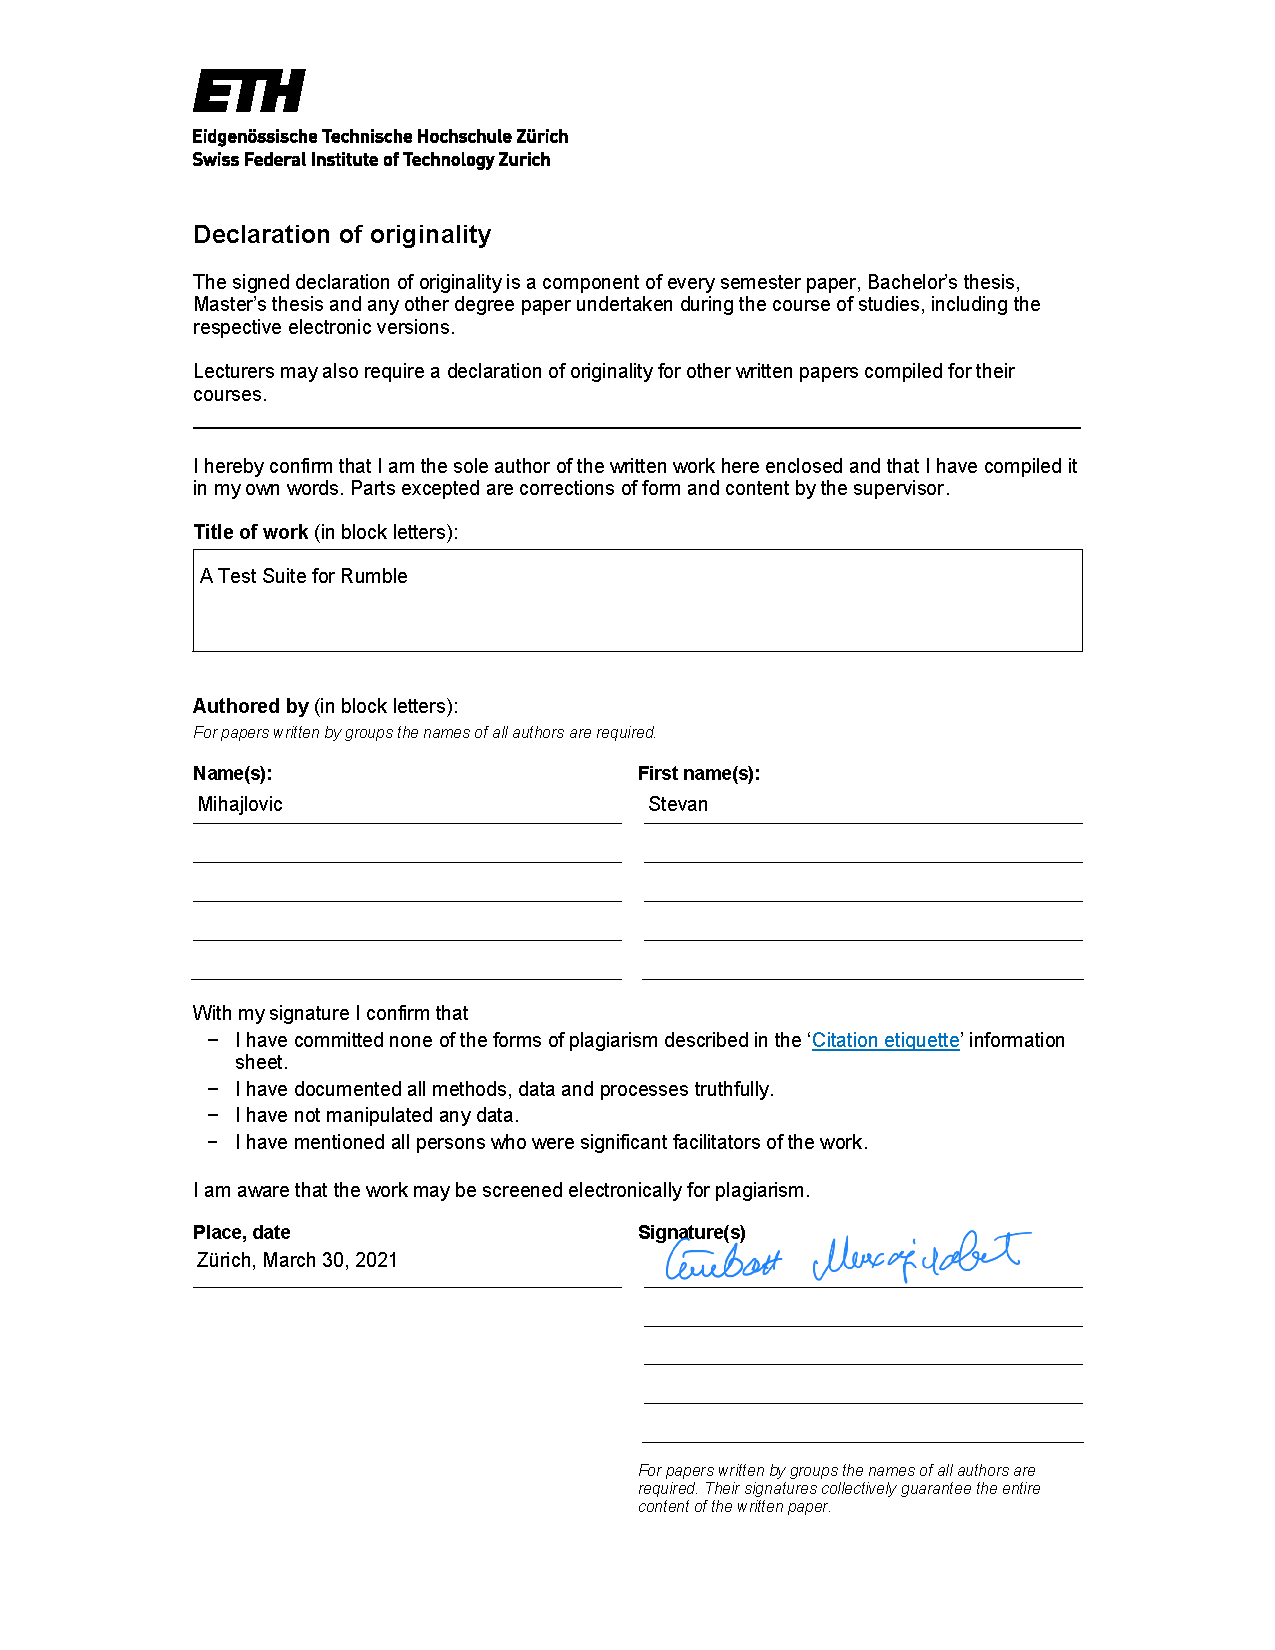
\includepdf[pages={-}]{declaration-originality.pdf}

\end{document}
